\documentclass[review]{elsarticle}

\usepackage{lineno,hyperref}
\modulolinenumbers[5]

\journal{Computer Physics Communications}

%%%%%%%%%%%%%%%%%%%%%%%
%% Elsevier bibliography styles
%%%%%%%%%%%%%%%%%%%%%%%
%% To change the style, put a % in front of the second line of the current style and
%% remove the % from the second line of the style you would like to use.
%%%%%%%%%%%%%%%%%%%%%%%

%% Numbered
%\bibliographystyle{model1-num-names}

%% Numbered without titles
%\bibliographystyle{model1a-num-names}

%% Harvard
%\bibliographystyle{model2-names.bst}\biboptions{authoryear}

%% Vancouver numbered
\usepackage{numcompress}
\bibliographystyle{model3-num-names}

%% Vancouver name/year
%\usepackage{numcompress}\bibliographystyle{model4-names}\biboptions{authoryear}

%% APA style
%\bibliographystyle{model5-names}\biboptions{authoryear}

%% AMA style
%\usepackage{numcompress}\bibliographystyle{model6-num-names}

\usepackage{graphicx}
\usepackage{caption}
\usepackage{subcaption}
\usepackage{amsmath}
\usepackage{amssymb}
\usepackage{amsthm}
\usepackage{color}
\usepackage{ifpdf}
\usepackage{booktabs} % For formal tables
\usepackage{listings}

%\setcopyright{rightsretained}

\newcommand{\up}{\vspace*{-1em}}
\newcommand{\upp}{\vspace*{-0.4em}}
\newcommand{\uppp}{\vspace*{-0.2em}}

\usepackage{hyperref}
\usepackage{float}
\usepackage[utf8]{inputenc}
\usepackage{multirow}
\usepackage{rotating}
\usepackage{setspace}
\usepackage{paralist}
\usepackage{makecell}
\usepackage{moresize}
\setlength{\textfloatsep}{5pt}
\usepackage{tabularx}
\usepackage{algorithm}
\usepackage{algpseudocode}

\usepackage{booktabs}
\usepackage{listings}
\usepackage{paralist}
\usepackage{wrapfig}
\usepackage{multirow}
\usepackage{ifpdf}
\usepackage{xspace}
\usepackage{keyval}
\usepackage{color}
\usepackage{nicefrac}
\usepackage{float}

\theoremstyle{definition}
\newtheorem{definition}{Definition}[section]

\usepackage{xcolor}
\usepackage{textcomp}

\definecolor{listinggray}{gray}{0.95}
\definecolor{darkgray}{gray}{0.7}
\definecolor{commentgreen}{rgb}{0, 0.4, 0}
\definecolor{darkblue}{rgb}{0, 0, 0.4}
\definecolor{middleblue}{rgb}{0, 0, 0.7}
\definecolor{darkred}{rgb}{0.4, 0, 0}
\definecolor{brown}{rgb}{0.5, 0.5, 0}

\usepackage[normalem]{ulem}
\def\cyanuwave{\bgroup \markoverwith{\lower3.5\p@\hbox{\sixly \textcolor{cyan}{\char58}}}\ULon}
\def\reduwave{\bgroup \markoverwith{\lower3.5\p@\hbox{\sixly \textcolor{red}{\char58}}}\ULon}
\def\blueuwave{\bgroup \markoverwith{\lower3.5\p@\hbox{\sixly \textcolor{blue}{\char58}}}\ULon}
\font\sixly=lasy6 % does not re-load if already loaded, so no memory problem.
\makeatother

% DOI
%\acmDOI{ }

% ISBN
%\acmISBN{ }


\newif\ifdraft
\drafttrue

\usepackage{adjustbox}
\usepackage{amsmath}
\renewcommand{\ttdefault}{pcr}
\usepackage{tabularx}

\usepackage{textcomp}
%\usepackage{natbib}
\setcitestyle{square, comma, numbers,sort&compress, super}
\usepackage{hypernat}
%\bibpunct{}{}{,}{s}{,}{,}
%% Remove brackets from numbering in List of References
\makeatletter
\renewcommand{\@biblabel}[1]{\quad#1.}
\makeatother
%% no space
\setlength{\bibsep}{0pt}

%% use \carriagereturn from dingbats 
% fix LaTeX Error: Command \checkmark already defined.
\let\checkmark\undefined
\usepackage{dingbat}
\usepackage{color}
\definecolor{mauve}{rgb}{0.58,0,0.82}
\definecolor{gray}{rgb}{0.5,0.5,0.5}
\renewcommand{\ttdefault}{pcr}
\usepackage{listings}

% Python style for highlighting
\newcommand\pythonstyle{\lstset{
    language=Python,
    basicstyle=\scriptsize\ttfamily,
    otherkeywords={self},             % Add keywords here
    keywordstyle=\bfseries\color{blue},
    emph={MyClass,__init__},          % Custom highlighting
    emphstyle=\ttfamily\bfseries\color{deepred},    % Custom highlighting style
    stringstyle=\color{mauve},
    commentstyle=\color{gray}\textit,      
    frame=tb,                         % Any extra options here
    showstringspaces=false,           %
    breaklines=true,
    prebreak=\carriagereturn,
    numberstyle=\tiny\color{gray},
    numbers=left,
    stepnumber=1
}}

% Python environment
\lstnewenvironment{python}[1][]
{
\pythonstyle
\lstset{#1}
}
{}

% Python for inline
\newcommand{\pythoninline[1]}{{\pythonstyle\lstinline!#1!}}

\usepackage{xspace}
\newcommand{\NaH}{Na$^{+}$/H$^{+}$\xspace}
\newcommand{\Na}{Na$^{+}$\xspace}
\newcommand{\Hp}{H$^{+}$\xspace}
\newcommand{\pKa}{\ensuremath{\mathrm{p}K_{\mathrm{a}}}\xspace}
\newcommand{\pK}{\ensuremath{\mathrm{p}K}}
\newcommand{\kon}{\ensuremath{k_{\text{on}}}}
\newcommand{\koff}{\ensuremath{k_{\text{off}}}}
\newcommand{\Aim}[1]{\textsc{Aim #1}\xspace}

\newcommand{\AIM}[2]{\paragraph{\Aim{#1}: #2}}

\newcommand{\PDB}[1]{PDB ID \textsc{#1}\xspace}


\newcommand{\nuvec}[1]{\boldsymbol{\nu}_{#1}}

\newcommand{\mus}{\ensuremath{\mu\text{s}}\xspace}

\newcommand{\package}[1]{\textsl{#1}}
\newcommand{\class}[1]{\textrm{#1}}

\newcommand{\tcomp}{\ensuremath{{t}_{\text{comp}}}\xspace}
\newcommand{\tIO}{\ensuremath{{t}_{\text{I/O}}}\xspace}
\newcommand{\tcomm}{\ensuremath{t_{\text{comm}}}\xspace}
\newcommand{\toverhead}{\ensuremath{t_{\text{overhead}}}\xspace}
%-------------------------------------------------------------------------------------------------------
\ifdraft
%\usepackage{textcomp}
\usepackage{xcolor}
\definecolor{ocolor}{rgb}{1,0,0.4}
\newcommand{\terminology}[1]{ {\textcolor{red} {(Terminology used: \textbf{#1}) }}}
\newcommand{\owave}[1]{ {\cyanuwave{#1}}}
\newcommand{\jwave}[1]{ {\reduwave{#1}}}
\newcommand{\alwave}[1]{ {\blueuwave{#1}}}
\newcommand{\jhanote}[1]{ {\textcolor{red} { ***shantenu: #1 }}}
\newcommand{\todo}[1]{ {\textcolor{brown} { TODO #1 }}}
\newcommand{\obnote}[1]{ {\textcolor{cyan} { ***oliver: #1 }}}
\definecolor{orange}{rgb}{1,.5,0}
\definecolor{dandelion}{cmyk}{0,0.29,0.84,0}
\newcommand{\mknote}[1]{ {\textcolor{blue} { ***mahzad: #1 }}}
\newcommand{\gpnote}[1]{{\textcolor{green} {***giannis: #1}}}
\newcommand{\note}[1]{ {\textcolor{magenta} { ***Note: #1 }}}
\else
\newcommand{\terminology}[1]{}
\newcommand{\jwave}[1]{#1}
\newcommand{\alnote}[1]{}
\newcommand{\mknote}[1]{}
\newcommand{\obnote}[1]{}
\newcommand{\rthreenote}[1]{}
\newcommand{\rfournote}[1]{}
\newcommand{\todo}[1]{}
\newcommand{\jhanote}[1]{}
\newcommand{\rtwonote}[1]{}
\newcommand{\gpnote}[1]{}
\newcommand{\note}[1]{}
\fi

\newcommand{\yarn}{YARN\xspace}
\newcommand{\rp}{RADICAL-Pilot\xspace}
\newcommand{\cloud}{cloud\xspace}
\newcommand{\clouds}{clouds\xspace}
\newcommand{\pilot}{Pilot\xspace}
\newcommand{\pilots}{Pilots\xspace}
\newcommand{\pilotjob}{Pilot-Job\xspace}
\newcommand{\pilotjobs}{Pilot-Jobs\xspace}
\newcommand{\pilotcompute}{Pilot-Compute\xspace}
\newcommand{\pilotcomputedescription}{Pilot-Compute Description\xspace}
\newcommand{\pilotdescription}{Pilot-Description\xspace}
\newcommand{\pilotcomputes}{Pilot-Computes\xspace}
\newcommand{\pilotdata}{Pilot-Data\xspace}
\newcommand{\pilotdatainmem}{Pilot-Data Memory\xspace}
\newcommand{\pilotdatadescription}{Pilot-Data Description\xspace}
\newcommand{\pilotdataservice}{Pilot-Data Service\xspace}
\newcommand{\pilotcomputeservice}{Pilot-Compute Service\xspace}
\newcommand{\computedataservice}{Compute-Data Service\xspace}
\newcommand{\computedatamanager}{Compute-Data Manager\xspace}
\newcommand{\computeunitdescription}{Compute-Unit Description\xspace}
\newcommand{\dataunitdescription}{Data-Unit Description\xspace}
\newcommand{\pilotmapreduce}{PilotMapReduce\xspace}
\newcommand{\mrmg}{MR-Manager\xspace}
\newcommand{\pstar}{P*\xspace}
\newcommand{\pd}{PD\xspace}
\newcommand{\pc}{PC\xspace}
\newcommand{\pcs}{PCs\xspace}
\newcommand{\pj}{PJ\xspace}
\newcommand{\pjs}{PJs\xspace}
\newcommand{\pds}{Pilot Data Service\xspace}
\newcommand{\computeunit}{Compute-Unit\xspace}
\newcommand{\computeunits}{Compute-Units\xspace}
\newcommand{\dataunit}{Data-Unit\xspace}
\newcommand{\dataunits}{Data-Units\xspace}
\newcommand{\du}{DU\xspace}
\newcommand{\dus}{DUs\xspace}
\newcommand{\dud}{DUD\xspace}
\newcommand{\cu}{CU\xspace}
\newcommand{\cus}{CUs\xspace}
\newcommand{\cud}{CUD\xspace}
\newcommand{\su}{SU\xspace}
\newcommand{\sus}{SUs\xspace}
\newcommand{\schedulableunit}{Schedulable Unit\xspace}
\newcommand{\schedulableunits}{Schedulable Units\xspace}
\newcommand{\cc}{c\&c\xspace}
\newcommand{\CC}{C\&C\xspace}

\newcommand{\numrep}{8 }
\newcommand{\samplenum}{4 }
\newcommand{\tmax}{$T_{max}$ }
\newcommand{\tc}{$T_{C}$ }
\newcommand{\tcnsp}{$T_{C}$}
\newcommand{\bj}{BigJob\xspace}
\newcommand{\irods}{iRODS\xspace}

\newcommand{\I}[1]{\textit{#1}\xspace}
\newcommand{\B}[1]{\textbf{#1}\xspace}
\newcommand{\T}[1]{\texttt{#1}\xspace}
%\newcommand{\C}[1]{\textsc{#1}\xspace}

% define a new float, with style `ruled`
\floatstyle{ruled}
\newfloat{scheme}{htbp}{lok}
\floatname{scheme}{Scheme}

%\lstdefinestyle{myListing}{
%    frame=single,
%    backgroundcolor=\color{listinggray},
    %float=t,
%    language=C,
%    basicstyle=\ttfamily \footnotesize,
%    breakautoindent=true,
%    breaklines=true
%    tabsize=2,
%    captionpos=b,
%    aboveskip=0em,
%    belowskip=-2em,
    %numbers=left,
    %numberstyle=\tiny
%}

%\lstdefinestyle{myPythonListing}{
%    frame=single,
%    backgroundcolor=\color{listinggray},
    %float=t,
%    language=Python,
%    basicstyle=\ttfamily \scriptsize,
%    breakautoindent=true,
%    breaklines=true
%    tabsize=2,
%    captionpos=b,
    %numbers=left,
    %numberstyle=\tiny
%}


\ifpdf
\DeclareGraphicsExtensions{.pdf, .jpg, .tif}
\else
\DeclareGraphicsExtensions{.ps,  .eps, .jpg}
\fi

\tolerance=1000
\hyphenpenalty=10


%\usepackage{listings}
%\usepackage{paralist}
% Python environment
%\lstnewenvironment{code}[1][]%
%{
%    \noindent
    %\minipage{0.98 \linewidth}
%    \minipage{1.0 \linewidth}
%    \vspace{0.5\baselineskip}
%   \lstset{
%        language=Python,
%       frame=single,
%        captionpos=b,
%        stringstyle=\ttfamily,
%        basicstyle=\scriptsize\ttfamily,
%        showstringspaces=false,#1}
%}
%{\endminipage}

\defaultleftmargin{1em}{}{}{}

%% `Elsevier LaTeX' style
%\bibliographystyle{elsarticle-num}
%%%%%%%%%%%%%%%%%%%%%%%

\begin{document}
\begin{frontmatter}    

\title{Guidelines on obtaining ideal Performance for Parallel Analysis of Molecular Dynamics Trajectories with Python on HPC Resources}

%% Group authors per affiliation:
\author[ASUphysics]{Mahzad Khoshlessan}
\ead{mkhoshle@asu.edu}

\author[Rutgers]{Ioannis Paraskevakos}
\ead{i.paraskev@rutgers.edu}

\author[IndianaDSC]{Geoffrey C. Fox}
\ead{gcf@indiana.edu}

\author[Rutgers]{Shantenu Jha}
\ead{shantenu.jha@rutgers.edu}

\author[ASUphysics,ASUCBP]{Oliver Beckstein\corref{correspondingauthor}}
\cortext[correspondingauthor]{Corresponding author}
\ead{oliver.beckstein@asu.edu}

\address[ASUphysics]{Department of Physics, Arizona State University,
  Tempe, AZ 85281, USA}
\address[ASUCBP]{Center for Biological Physics, Arizona State University,
  Tempe, AZ 85281, USA}
\address[Rutgers]{Department of Electrical \& Computer Engineering,
  Rutgers University, Piscataway, NJ 08854, USA}
\address[IndianaDSC]{Digital Science Center, Indiana University,
  Bloomington, IN 47405}

%\renewcommand{\shortauthors}{M. Khoshlessan et al.}
    
\begin{abstract} 
Typical size of the molecular dynamics (MD) trajectories from data-intensive bio-molecular simulations ranges from gigabytes to terabytes. 
However, the computational biophysics community misses effective use of high performance computing (HPC) resources for efficiently analyzing these trajectories and more importantly achieving linear scaling still remains a big challenge. 
\obnote{We will have to be a bit more careful how we phrase this because VMD can analyze on thousands of cores and cpptraj is apparently also doing pretty well. There is also HiMach.Benchmarks, however, are scarce.}
\mknote{Need to make clear how this work distinguishes from their work}
Present work aims to provide insights, guidelines and strategies to the community on how to take advantage of the available HPC resources to gain the best possible performance.
We investigated a single program multiple data (SPMD) execution model where each process executes the same program, to parallelize the Map-Reduce Root Mean Square Distance (RMSD) and Dihedral Featurization algorithms for analysis of MD trajectories in the MDAnalysis library. \gpnote{I am not sure RMSD can be stated as a MR algorithm. We do not employ any reduce
function to provide a single answer for the whole dataset. Am I missing something? }\mknote{No, but at the end we are gathering the data from all ranks to rank 0. Oliver believed that this can be considered as a MR too!}
We employ the Python language because it is widely used in the bio-molecular simulation field and focus on an MPI-based implementations.  
We notice that straggler tasks negatively impact the performance and act as scalability bottlenecks. 
Straggler tasks are a very common problem in heterogeneous environments and are significantly slower than the mean execution time of all tasks, impeding job completion time.
Our initial analysis shows that accessing a single file on the distributed file system leads to stragglers, and as a result, prevents any scaling beyond one node.
We introduce an important performance parameter $t_{Compute}$/$t_{IO}$ which determines whether we observe any stragglers.
In addition, we show that there are two factors that lead to stragglers including I/O and communication. 
Taking advantage of Global Arrays (GA) toolkit we have been able to obtain significant improvement in communication cost and performance.
In addition, we show two different approaches to overcome the I/O bottleneck and compare their performance. 
First approach is splitting the trajectory into as many trajectory segments as number of processes.
The second approach is through MPI-based approach using Parallel HDF5 where we examine the performance differences between both collective and independent I/O.
Applying these strategies, we obtained near ideal scaling and performance.  
\end{abstract}

%\keywords{Data analytics, MD Simulations Analysis, Parallel MD analysis, task-parallel}


\begin{keyword}
Python\sep MPI\sep HPC\sep MDAnalysis\sep Global Array\sep MPI I/O\sep Straggler\sep Molecular Dynamic
\MSC[2010] 00-01\sep  99-00
\end{keyword}

\end{frontmatter}

\linenumbers

\section{Introduction}
\label{sec:introduction}
The increase in computational power coupled with sophisticated algorithms has lead rapid increase in the amount of data produced by MD simulations. 
Typical trajectory sizes from MD simulations range from gigabytes to terabytes. 
Therefore, analyzing these trajectories has become a very tedious process in many workflows and as a result people are trying to look for state of the art HPC tools (MPI and OpenMP) or Big Data ecosystem to tackle this problem.
The need for parallel programming and running these programs on parallel architectures is obvious, however, efficiently programming for a parallel environment can be a very daunting task. 

\package{MDAnalysis} \citep{Gowers:2016aa,Michaud-Agrawal:2011fu} is a widely used open-source Python library to analyze molecular dynamics (MD) simulations. 
\package{MDAnalysis} allows analysis of different file formats for trajectories generated by various packages for molecular dynamic simulations. 

In our previous study, we used a parallel map-reduce approach to study the performance of RMSD task \cite{Khoshlessan:2017ab}. 
We previously looked at the \package{Dask} library \cite{Rocklin:2015aa}, which splits a computation in tasks and generates directed acyclic graphs (DAG) of these tasks that can be executed on a range of schedulers. 
We also implemented the parallel analysis scheme with MPI, using the \package{mpi4py} package \cite{Dalcin:2011aa, Dalcin:2005aa}. 
For both Dask and MPI we found that our benchmark task, the calculation of the minimum C$_{\alpha}$ RMSD for a
subset of the residues in the enzyme adenylate kinase from a long MD simulation, only showed good strong scaling within a single node (up
to 24 cores on \emph{SDSC Comet}).
However, with a single compute node we are limited by the resources for executing a given problem.
Distributed computing, allows parallelizing our problems for larger problem sizes and lead to performance gains.
But, as soon as we extend the computation beyond a single node, performance drops due to \emph{stragglers} tasks, a subset of Dask worker processes or MPI ranks that are significantly slower than the mean execution time of all tasks, increasing the total time to solution.
Stragglers significantly impede job completion time and are a big challenge toward achieving improved performance.

MPI should have, in principle, close to ideal scaling for a pleasingly parallel task such as the analysis of trajectory blocks, and does not require additional considerations of, e.g., scheduler performance as for Dask. 
Therefore, in the present study, we analyze the MPI case in more detail to better understand the origin of the stragglers.

We want to provide simple and robust parallelization approaches to analyzing molecular dynamics (MD) trajectories, in order to remove a narrowing bottle neck in the bio-molecular simulation field. 
We have selected two of the most common map-reduce algorithms in \package{MDAnalysis} one of which is I/O bound and the other is compute bound.
We use SPMD paradigm to parallelize theses two algorithms on HPC resources.
With SPMD, each process executes essentially the same code but on a different part of the data. 
We use Python, a machine-independent, byte-code interpreted, object-oriented programming (OOP) language, which is well-established in HPC parallel environments \cite{GAiN}. 
Based on our initial analysis there is an important performance parameter,  $t_{Compute}$/$t_{IO}$, that determines whether we observe stragglers.
We show this behavior using RMSD and dihedral featurization algorithms.
If $t_{Compute}$/$t_{IO}$  $\gg 1$, the algorithm scales very well, otherwise it does not scale beyond one node. 
For the algorithms with small $t_{Compute}$/$t_{IO}$, we need to come up with strategies to improve scaling and overcome straggler problems.
Looking at the timing distribution across all ranks we noticed that communication and I/O are the two main scalability bottlenecks.
Taking advantage of Global Array toolkit \cite{GA}, each rank places its data in shared memory which allows direct access using the global address space rather than through a message-passing protocol. 
This reduces communication cost noticeably.
Although Global Array toolkit is very helpful for improving the performance it is still not enough because I/O remains a bottleneck.
Our data shows that I/O time does not scale beyond one node. 
Due to the large file size and memory limit, processes are not able to load the whole trajectory into memory at once, and as a result each process is only allowed to load one frame into memory at a time.
Therefore, with large number of frames, there will be a lot of file access requests and when the compute time is small with respect to I/O, then I/O can be a major issue.
Hence, we needed to find ways to improve I/O scaling beyond a single compute node.
In order to improve I/O scaling, we came up with two approaches: MPI-based approach using Parallel HDF5 \cite{pythonhdf5}, and splitting our trajectory to as many trajectory segments as the number of processes. 
We provide the detail on these approaches on the following sections.
But, both approaches significantly improved the performance and we were able to achieve near ideal scaling.

\section{Background \& Related Works}
\label{background}
\mknote{I have another idea. We can compare the performance of cpptraj with our approach for two cases of large and small tcomp/tIO. Especially we can see if cpptraj can be scaled when tcomp/tIo is small (i.e. I/O bound jobs)}
\gpnote{You brought the related work from the workshop paper here, but still you left CPPTraj and HiMach. Either remove them or show what is that you ae doing different.}

Long Tail phenomena, whereby a small proportion of task stragglers significantly impede job completion time is a big challenge toward achieving improved performance \cite{Garraghan2016}.
Over the past few years a significant amount of research has been done trying to detect and mitigate stragglers \cite{Rosen2012, Dean2004, Chen2014, Bhandare2016, Kwon2012}. 
There are also works to find the stragglers root-cause in many big data processing systems \cite{Ballani2011, Ananthanarayanan2014, Jeyakumar2013, Li2014, Zaharia2012}.

Straggler root-cause has both internal and external factors. 
Internal factors include heterogeneous capacity of worker nodes, and resource competition due to other tasks running on the same worker node. 
External factors include resource competition due to co-hosted applications, input data skew, remote input or output source being too slow and faulty hardware \cite{Chen2014}.

Spark introduces stragglers for a number of different reasons: 1) garbage collections~\cite{Kyong2017,Ousterhout2017}, 2) JVM positioning to cores~\cite{Kyong2017}, 
2) the delay's introduced while the task moves from the scheduler to executing~\cite{Gittens2016}, 3) Disk I/O during shuffling, 4) Java's just-in-time compilation~\cite{Ousterhout2017}, 
and 5) output skew \cite{Ousterhout2017}. 
In addition to these reasons, stragglers on Spark have been attributed to the overall performance of the worker or competition between resources \cite{Yang2016}.

Tuning resource allocation and tuning parallelism are other methods to improve Spark job performance. 
However, manual tuning are laborious and imprecise. 
Many frameworks suggest breaking the workload into many small tasks that are dynamically scheduled at runtime \cite{Rosen2012}. 
This approach is only effective in systems with high-throughput, low-latency task schedulers and efficient data materialization though.
In general, finer-grained splitting produces fewer stragglers; however, at some point the overhead of a large number of splits starts to dominate. 

Some frameworks will identify the straggler nodes using a slow Node-Threshold. 
They identify straggler node when its performance score is less than the average performance score of all nodes and therefore prevent to launch any tasks on these slow nodes. 
The straggler node can be due to the faulty hardware or mis-configuration \cite{Dean2004}. 
However, this solution only addresses hardware-based stragglers \cite{Chen2014}.

For most of the factors causing stragglers, speculative execution and its improved versions are an effective way to solve the straggler problem. 
Speculative execution (back-up tasks) is a replication-based reactive straggler mitigation technique that spawns redundant copies of the slow running tasks, hoping a copy will reach completion before the original. 
This is the most prominently used in production clusters at Facebook and Microsoft Bing and is also implemented by both Hadoop and Google\textsc{\char13}s MapReduce \cite{Dean2004}.
Google reported that speculative execution can improve job running times by $44\%$ \cite{Dean2004}.
However, without any additional information, such reactive techniques can not differentiate between nodes that are inherently slow and nodes that are temporarily overloaded (i.e. input data skew or data imbalance) \cite{Chen2014, Bhandare2016}.

Sampling or similar techniques can help estimate the data distribution to split the data more evenly. 
However, such statistics are often expensive to collect, insufficiently precise, or obsolete. 
Moreover, stragglers can happen even if the data distribution is balanced, due to unbalanced processing complexity for different parts of the data \cite{Khoshlessan:2017ab}.

SkewTune is another technique for addressing data imbalance. 
SkewTune identifies the task with the greatest expected remaining processing time when a node becomes idle. 
The un-processed input data of this straggling task is then pro-actively repartitioned in a way that fully utilizes the nodes in the cluster and preserves 
the ordering of the input data so that the original output can be reconstructed by concatenation \cite{Kwon2012}. 
SkewTune can significantly reduce job runtime and adds little to no overhead in the absence of skew; however, the cost of fully reading the rest of a straggler's input can be prohibitive, in particular, making 
the technique meaningless if the straggler was already dominated by the cost of reading the input.

Garraghan et al. \cite{Garraghan2016} studied stragglers on Virtualized Cloud Data-centers. 
Through statistical analysis they found that the most frequent reasons were high CPU utilization, disk utilization, unhandled I/O access requests and network package loss. 
About $3\%$ to $6.5\%$ of the tasks were stragglers resulting to a $37.8\%$ to almost $50\%$ of jobs negatively impacted. 
In this study, task stragglers are defined as tasks whose execution is $150\%$ of the median duration of all tasks within the same job and median task duration is used instead of mean task duration. 
This is especially because median job execution duration is less affected by extreme execution times caused by stragglers.  

The analysis performed on the trace data from Microsoft Bing's production cluster shows that $80\%$ of stragglers have a uniform probability of delay between $150-250\%$ 
compared to the median task duration, with 10\% exhibiting a delay $1000\%$ greater than median task duration \cite{Ananthanarayanan2010}.

Cloud data-flow deals with stragglers problem using dynamic work rebalancing. 
However, this method has its own technical challenges which includes data consistency, intense systematic testing, as well as a careful design, and predicting how a task will progress over time \cite{Schmidt2016}.
In addition, this approach is only effective in systems with high-throughput, low-latency task schedulers and efficient data materialization \cite{Rosen2012}.

Blocked time analysis is used to measure how long each task spends blocked on a given resource. 
These approach provides a per-task measurements and allows the understanding of straggler root-causes by correlating slow tasks with long blocked times \cite{Ousterhout2015}. 
However, the work by \cite{Ousterhout2015} does not look at a vast range of workloads nor a wide range of cluster sizes.

Intelligent scheduling [AWE-WQ] is another approach to remove stragglers. Several components of task scheduling affect the scalability.
The first is knowledge of a worker\textsc{\char13}s past task execution times. This allows to schedule tasks preferentially to the most performant machines. 
The second involves task replication to remove the effect of straggling workers. 
By monitoring the state of the workers either busy or idle ($w_{i}$) and the number of tasks waiting to be assigned a worker, task replication can be engaged when $w_{i}>0$.

All of these previous studies are trying to mitigate stragglers through a wide variety of approaches.
While a comprehensive solution will involve tricks to avoid causing stragglers. 
This work focuses on the stragglers root-causes that prevent us from achieving near ideal scaling in \package{MDAnalysis} beyond a single compute node.
In the present study, we are trying to find the root-cause of the straggler tasks and solutions through which we can improve performance and scaling.



\section{Molecular Dynamics Analysis Applications}
\label{use_cases}

\subsection{MDAnalysis}
Simulation data exist in trajectories in the form of three dimensional time series (atoms positions and velocities), and these come in a plethora of different and idiosyncratic file formats. 
\package{MDAnalysis} is a widely used open source Python library to analyze these trajectory files with an object oriented interface. 
The package is written in Python (compatible with version 2.7 and 3.4+), with time critical code in C/Cython. 
\label{sec:mda}

\subsubsection{Root Mean Square Distance (RMSD)}
The calculation of the root mean square distance (\textbf{RMSD}) for C$_{\alpha}$ atoms after
optimal superposition with the QCPROT algorithm \cite{Liu:2010kx,Theobald:2005vn} is commonly required in the analysis of molecular dynamics simulations (Algorithm \ref{alg:RMSD}). 
The task used for the purpose of our benchmark is the $RMSD=\sqrt{\frac{1}{N}\sum_{i=1}^{N}\delta_{i}^{2}}$ implemented in MDAnalysis.analysis.rms module where $\delta_{i}$ is the distance between atom i and a reference structure (implemented in Cython \cite{Gowers:2016aa}).  
This function computes the RMSD between two sets of coordinates using the fast QCPROT algorithm to optimally superimpose two structures and then calculates the RMSD. 

To this, the protein structure (selected C$_{\alpha}$ atoms) in the initial frame will be considered as the reference and as the mobile group at other time steps. 
The superposition is done in the following way:
First, the mobile group is translated so that its center of mass coincides with the one of reference. 
Second, a rotation matrix is computed that spatially aligns the mobile group to reference which minimizes the RMSD between the coordinates of the mobile group and reference structure. 
Finally, all atoms in mobile group are shifted and rotated.
For each frame, a non-negative floating point number is calculated and the final result is a time-series of the RMSD. 
RMSD values show how rigid the domains in a protein structure are, during the transition. 
The order of complexity for RMSD algorithm \ref{alg:RMSD} is $\mathcal{O}(T \times N^{2})$ \cite{rmsd} where T is the number of frames in the trajectory and N the number of particles in a 
frame.

\begin{algorithm}[ht!]
	\scriptsize
	\caption{MPI-parallel Multi-frame RMSD Algorithm}
	\label{alg:RMSD}
	\hspace*{\algorithmicindent} \textbf{Input:} \emph{size}: Total number of frames \\
	\hspace*{\algorithmicindent} \emph{ref}: mobile group in the initial frame which will be considered as reference \\
	\hspace*{\algorithmicindent} \emph{start \& stop}: Starting and stopping frame index\\
	\hspace*{\algorithmicindent} \emph{topology \& trajectory}: files to read the data structure from \\
	\hspace*{\algorithmicindent} \textbf{Output:} Calculated RMSD arrays
	\begin{algorithmic}[1]
		\Procedure{$Block\_RMSD$}{topology, trajectory, $ref$, start, stop}                       
		\State u $\leftarrow$ Universe(topology, trajectory)\Comment{u hold all the information of the physical system}
		\State $g$ $\leftarrow$ u.frames[start:stop]
		\For{$\forall iframe$ in $g$}
		\State $results[iframe] \leftarrow RMSD(g, ref)$
		\EndFor
		\State \Return results
		\EndProcedure
		\\        
		\State MPI Init
		\State rank $\leftarrow$ rank ID
		\State index $\leftarrow$ indices of mobile atom group
		\State xref0 $\leftarrow$ Reference atom group\textsc{\char13}s position
		\State out $\leftarrow$ Block\_RMSD(topology, trajectory, xref0, start=start, stop=stop)
		\\
		\State Gather(out, RMSD\_data, rank\_ID=0)
		\State MPI Finalize
	\end{algorithmic}
\end{algorithm}

\subsubsection{Dihedral Featurization}
As a real-world compute-bound task we investigated \textbf{Dihedral featurization} \cite{Sittel:2014aa} (Algorithm \ref{alg:Dihedral}) whereby a time series of
feature vectors consisting of the two backbone dihedral angles per residue ($\phi_{i}$ and $\psi_{i}$) is calculated for all 212
non-terminal residues. For each frame, an array of dihedral angles is calculated where for later convenience, an angle $\theta_{i}$ is
actually represented as $(\cos\theta_{i}, \sin\theta_{i})$. 
The order of complexity for Dihedral featurization algorithm (Algorithm \ref{alg:Dihedral}) is $\mathcal{O}(T \times N)$. 
\obnote{Write out the calculation, based on the 4 atoms}
\mknote{What calculations? how residues are converted to dihedrals? or the procedure we perform in the algorithm? that one is explained in algorithm 2}

\begin{algorithm}[ht!]
	\scriptsize
	\caption{MPI-parallel Multi-frame Dihedral Featurization Algorithm}
	\label{alg:Dihedral}
	\hspace*{\algorithmicindent} \textbf{Input:} \emph{mobile}: the desired atom groups to perform RMSD on them \\ 
	\hspace*{\algorithmicindent} \emph{start \& stop}: that tell which block of trajectory (frames) is assigned to each rank \\
	\hspace*{\algorithmicindent} \emph{topology \& trajectory}: files to read the data structure from \\
	\hspace*{\algorithmicindent} \textbf{Output:} Calculated Dihedral Angles
	\begin{algorithmic}[1]
		\Procedure{$angle2sincos$}{x}     
		\State \Return $\cos{x},\: \sin{x}$
		\EndProcedure
		\\
		\Procedure{$residues\_to\_dihedrals$}{residues}
		\State List angles
		\For{$\forall res$ in $residues$}
		\State Append $(\phi (res),\: \psi (res))$ in angles
		\EndFor
		\State \Return angles
		\EndProcedure
		\\
		\Procedure{$featurize\_dihedrals$}{dihedrals}
		\State List angles
		\For{$\forall dihedral$ in $dihedrals$}
		\State Append value of $dihedral$ in angles
		\EndFor
		\State \Return \texttt{angle2sincos(angles)}
		\EndProcedure
		\\
		\Procedure{$Block\_Dihedral$}{topology, trajectory, $ref$, start, stop}                       
		\State u $\leftarrow$ Universe(topology, trajectory)
		\State $g$ $\leftarrow$ u.frames[start:stop]
		\State List $results$
		\For{$\forall frame$ in $g$}
		\State $D_{angles} \leftarrow featurize\_dihedrals(dihedrals)$
		\State Append $D_{angles}$ in $results$ 
		\EndFor
		\EndProcedure
		\\      
		\State MPI Init 
		\State residues $\leftarrow$ residues of mobile atom group
		\State dihedrals $\leftarrow$ residues\_to\_dihedrals(residues)
		\State rank $\leftarrow$ rank ID
		\State index $\leftarrow$ indices of mobile atom group
		\State xref0 $\leftarrow$ Reference atom group\textsc{\char13}s position
		\State out $\leftarrow$ Block\_Dihedral(topology, trajectory, xref0, start=start, stop=stop)
		\\
		\State Gather(out, RMSD\_data, rank\_ID=0)
		\State MPI Finalize
	\end{algorithmic}
\end{algorithm}

\subsection{MPI for Python \package{mpi4py}}
MPI for Python (\package{mpi4py}) is a Python wrapper written over Message Passing Interface (MPI) standard and allows any Python program to employ multiple processors \cite{Dalcin:2011aa, Dalcin:2005aa}.
Python has several advantages that makes it a very attractive language including rapid development of small scripts and code prototypes as well as large applications and highly portable and reusable modules and libraries.
\gpnote{I do not understand this sentence. What do you mean by other factors?}\mknote{I say other factors like LOC, number of function invocation, ..}
In addition, Python\textsc{\char13}s interactive nature, and other factors like lines of codes (LOC), number of function invocation, and development time adds to its attractiveness and clarifies why it is a good investment to extend Python use to message-passing parallel programming applications.
Based on the efficiency tests \cite{Dalcin:2011aa, Dalcin:2005aa}, the performance degradation due to using \package{mpi4py} is not prohibitive and the overhead introduced by \package{mpi4py} is far smaller than the overhead associated to the use of interpreted versus compiled languages \cite{GAiN}.
In addition, there are works on improving the communication performance in \package{mpi4py} and it shows minimal overheads compared to C code if efficient raw memory buffers are used for communication \cite{Dalcin:2011aa}.

\subsection{Applications of Global Array}
Global array toolkit provides users with a language interface that allows them to distribute data while maintaining the type of global index space and programming syntax similar to what is available when programming on a single processor \cite{GA}.

Global array (GA) toolkit allows manipulating physically distributed dense multi-dimensional arrays without explicitly defining communication and synchronization between processes.
Global Arrays in NumPy (GAiN) extends GA to python through Numpy \cite{GAiN}. 
The basic components of the Global Arrays toolkit are function calls to create global arrays ($ga\_create$), copy data to ($ga\_put$), from ($ga\_get$), and between global arrays ($ga\_distribution$, $ga\_scatter$), and identify and access the portions of the global array data that are held locally ($ga\_access$). 
In addition, there are also functions to destroy arrays ($ga\_destroy$) and free up the memory originally allocated to them \cite{GAiN}.

The global array itself is physically located in the local memory space of each process \cite{GA}. 
User can get a pointer to this memory by using ga\_access function or one of its variants.
Using this pointer it is possible to directly modify the data that is local to each process.
The GA library keeps track of all these memory locations by recording a list\gpnote{Is this list distributed of centralized? Which process is the owner?}\mknote{All the processes have access to it and in that way will get aware of any change in the data of other processes} of them when a global array is created. 
When a process tries to access a block of data, it first does a decomposition of the request into individual blocks representing the contribution to the total request from the data held locally on each process \cite{PNNL:2018}. 
The requesting process then makes individual requests to each of the remote processes. 
The requests are implemented using the native one-sided semantics inside the the infini-band Verbs library. 
OpenIB/infini-band uses SHMEM (Symmetric Hierarchical MEMory) parallel computing library \gpnote{You want to avoid language that is OS specific. You say in the introduction that scientist are not system administrators. sys5 shmem is very specific even for me.}\mknote{tried to make it less specific} within the node and will use the infini-band network card to communicate between nodes.
Algorithm \ref{alg:GA} describes RMSD algorithm in combination with the global array.
In this algorithm, we use global array instead of message passage paradigm to see if we can reduce communication cost. 

\begin{algorithm}[ht!]
	\scriptsize
	\caption{MPI-parallel Multi-frame RMSD using Global Arrays}
	\label{alg:GA}
	\hspace*{\algorithmicindent} \textbf{Input:}\emph{size}: Total number of frames assigned to each rank $N_{b}$\\
	\hspace*{\algorithmicindent} \emph{g\_a}: Initialized global array \\
	\hspace*{\algorithmicindent} \emph{xref0}: mobile group in the initial frame which will be considered as rerference \\
	\hspace*{\algorithmicindent} \emph{start \& stop}: that tell which block of trajectory (frames) is assigned to each rank \\
	\hspace*{\algorithmicindent} \emph{topology \& trajectory}: files to read the data structure from \\
	\hspace*{\algorithmicindent}\textbf{Include:} $Block\_RMSD$ from Algorithm \ref{alg:RMSD}
	\begin{algorithmic}[1]
		
		\State bsize $\leftarrow$ ceil(trajectory.number\_frames / size)
		\State g\_a $\leftarrow$ ga.create(ga.C\_DBL, [bsize*size,2], "RMSD")
		\State buf $\leftarrow$ np.zeros([bsize*size,2], dtype=float)
		\State out $\leftarrow$ Block\_RMSD(topology, trajectory, xref0, start=start, stop=stop)
		\State ga.put(g\_a, out, (start,0), (stop,2))
		\If{rank == 0}
		\State buf $\leftarrow$ ga.get(g\_a, lo=None, hi=None)
		\EndIf
	\end{algorithmic}
\end{algorithm}

\subsection{MPI and Parallel HDF5}
MPI-based applications work by launching multiple parallel instances of the Python interpreter which communicate with each other via the MPI library. 
HDF5\gpnote{This is a very nice oportunity to introduce HDF5. More details about HDF5 would be nice. If you assume that the reader does not know MPI4py, most probably will not know HDF5} itself handles nearly all the details involved with coordinating file access through MPI library.
This is advantageous to avoid multiple processes to compete over accessing the same file on disk\gpnote{I am not sure what you want to say here. Are the processes accessing the file atomically, i.e. when on process access it all others are blocked? Doesn't that defeat the purpose of parallel I/O}. \mknote{Previously I had more detail in this section and Oliver suggested to summarize and avoid too much detail. What type of info do you think will be good to be added here?}
In fact in python, MPI-IO opens shared files with a mpio driver. 
In addition,  MPI communicator should be supplied as well and the users also need to follow some constraints for data consistency \cite{pythonhdf5}.

\subsubsection{Collective Versus Independent Operations} 
MPI has two flavors of operation: collective, which means that all processes have to participate in the same order, and independent, which means each process can perform the operation or not and the order also does not matter  \cite{pythonhdf5}.
With HDF5, modifications to file metadata must be done collectively and although all processes perform the same task, they do not wait until the others catch up \cite{pythonhdf5}. 
Other tasks and any type of data operations can be performed independently by processes.
In the present study, we use independent operations.


\section{Benchmark Environment}
\label{system}
The test system contained the protein adenylate kinase with 214 amino acid residues and 3341 atoms in total \cite{Seyler:2014il}. 
The trajectory \cite{Seyler:2017aa} was in Gromacs XTC format trajectory (``600x'' in \citet{Khoshlessan:2017ab}) with a size of about 30 GB and 2,512,200
time frames (corresponding to $602.4 \sim \mu s$ simulated time) which represents a typical medium per-frame size but is very long for
current standards.

The experiments were executed on the XSEDE Supercomputers: \emph{SDSC Comet}, 
\emph{PSC Bridges} and \emph{SuperMIC}. SDSC Comet is a 2.7 PFlop/s cluster with 
6,400 compute nodes in total. The standard compute nodes consist of Intel Xeon 
E5-2680v3 processors, 128 GB DDR4 DRAM (64 GB per socket). The network topology 
is 56 Gbps FDR Infini-Band (IB).

PSC Bridges is a 1.35 PFlop/s cluster with four types of computational nodes. Bridges 
computational nodes supply 1.3018 PFlop/s and 274 TiB RAM. The Regular Shared 
Memory (RSM) nodes consist of Intel Haswell (E5-2695 v3) processors, 128 GB DDR4 
DRAM (64 GB per socket). The network topology is 12.37 Gbps Omni-Path Architecture 
(OPA).

LSU SuperMIC offers 360 compute nodes with Ivy Bridge Intel processors (E5-2680).
Each node has 64 GBs DDR3 RAM. SUperMIC's nodes are connected 56 Gbps Infiniband 
Network. In addition, it offers 20 hybrid nodes which provide an NVIDIA GPU. SuperMIC's
peak performance is measured at 557 TFlop/s.
All the experiments are performed using standard compute nodes on Comet, PSC Bridges and SuperMIC respectively in the present study.
 \gpnote{The RSM nodes on Bridges are compute nodes as well. I suggest you say standard compute nodes 
for Comet. Also, you may need to say what other types of nodes do they offer, 
because the naming is very specific. Otherwis, just introduce the nodes you used.}
\mknote{Ok I used standard compute node for all clusters. I think because we have not used other types of nodes it is better to not mention them.
Anyway they are not related.}

\begin{table}[ht!]
	\centering
	\begin{adjustbox}{max width=\textwidth}
		\begin{tabular}{c c c c c c c c}
			\toprule
			\bfseries\thead{Cluster} & \bfseries\thead{Nodes} & \bfseries\thead{Number} & \bfseries\thead{CPUs} &  \bfseries\thead{RAM} & \bfseries\thead{Network Topology} & \makecell{\bfseries\thead{Scheduler and  \\ Resource Manager}}\\
			\midrule
			\bfseries SDSC Comet & Compute & 6400 & \makecell{2 Intel Xeon (E5-2680v3) CPUs \\ 12 cores/CPU, 2.5 GHz} &128 GB DDR4 DRAM & 56 Gbps IB & SLURM\\
			\bfseries PSC Bridges & RSM & 752 & \makecell{2 Intel Haswell (E5-2695 v3) CPUs \\14 cores/CPU, 2.3 GHz} & 128 GB, DDR4-2133Mhz & 12.37 Gbps OPA & SLURM\\
			\bfseries SuperMIC & Standard & 360 & \makecell{2 Intel Ivy Bridges (E5-2680) CPUs \\10 cores/CPU, 2.8GB GHz} & 64 GB, DDR3-1866Mhz  & 56Gbps IB & PBS\\
			\bottomrule
		\end{tabular}
	\end{adjustbox}
	\caption[System configuration used in the present study]
	{List of benchmarked clusters and their system configuration}
	\label{tab:sys-config}
\end{table}

\subsection{Installing libraries on multi-user HPC systems}
\obnote{Include table with software and versions; add a paragraph in which you mention software, summarize how it was compiled, and reference the table.}
\mknote{Are the following enough?}
Different packages and libraries are used in the present study in order to achieve the desired performance. 
However, getting scientific libraries installed can be a very challenging task.
Lack of documentation and good software engineering practices, non-standard installation procedures, and lots of dependencies can contribute to the challenge of getting the libraries to work [???].
Scientists mostly care about the science and they are often not software engineers or system administrators. 
Therefore, the libraries and tools they need should be easily accessible. 
This is not always the case, though.

In fact, many domain specific packages are not available through package manager in supercomputers and as a result,
we spent considerable amount of time getting packages dependencies to work in the process of our performance study.
As a result, we provide detail information on how we managed to build these libraries.
This will let future works spend least amount of time for this purpose. 
Detailed information regarding the version of each library, its dependencies, the quality of its documentation, the time necessary for building and installing the packages are given in Table \ref{tab:version}. 

\begin{table}[ht!]
\centering
\begin{adjustbox}{max width=\textwidth}
\begin{tabular}{c c c c c c c}
  \toprule
            \bfseries\thead{Package} & \bfseries\thead{Version} & \bfseries\thead{Description} & \bfseries\thead{Time to Result} & \bfseries\thead{Documentation} & \bfseries\thead{Installation} & \bfseries\thead{Dependencies}\\
  \midrule
   \bfseries GCC & 4.9.4 & GNU Compiler Collection & Fast & Excellent & \makecell{via configuration \\files, environment \\or command line options, \\ minimal configuration \\ is required} &--\\
   \bfseries OpenMPI & 1.10.7 & MPI Implementation & Fast & Excellent & \makecell{via configuration \\ files, environment \\or command line options, \\ minimal configuration \\ is required} &--\\
   \bfseries Global Array & 5.6.1 & Global Array & Slow & Good & \makecell{via configuration files, environment \\or command line options, \\ several optional configuration\\ settings available} &\makecell{MPI 1.x/2.x/3.x \\ implementation like \\ MPICH or Open MPI \\ built with shared/dynamic\\ libraries, GCC}\\
   \bfseries MPI4py & 3.0.0 & MPI for Python & Very Fast & Excellent & Conda Installation &\makecell{Python 2.7, \\or above, \\ MPI 1.x/2.x/3.x  \\ implementation like \\ MPICH or Open-MPI \\built with shared/dynamic \\libraries, Cython}\\
   \bfseries GA4py & 1.0 & Global Array for Python & Fast & Average & Python Setuptools &\makecell{Python 2.7, \\or above, \\ MPI 1.x/2.x/3.x  \\implementation like \\ MPICH or Open-MPI \\ built with shared/dynamic \\libraries, Cython,  \\MPI4py, Numpy} \\
   \bfseries PHDF5 & 1.10.1 & Parallel HDF5 & Slow & Excellent & \makecell{via configuration files, environment \\or command line options, \\ several optional configuration\\ settings available} &\makecell{MPI 1.x/2.x/3.x  \\ implementation like \\ MPICH or Open-MPI,  \\GNU, MPIF90,  \\MPICC, MPICXX}\\
   \bfseries H5py &  2.7.1 & Pythonic wrapper around the HDF5 & Very Fast & Excellent & Conda Installation & \makecell{Python 2.7, or above,\\ PHDF5, Cython}\\    
   \bfseries MDAnalysis & 0.17.0 & \makecell{Python library  \\ to analyze  \\trajectories from  \\MD simulations} & Very Fast & Excellent & Conda Installation & \makecell{Python $>=$2.7, or $<$3,\\ Cython, GNU, \\Numpy}\\
  \bottomrule
\end{tabular}
\end{adjustbox}
\caption[Version of the packages used in the present study]
{Detailed comparison on the dependency and installation of different packages used in the present study on multi-user HPC systems}
\label{tab:version}
\end{table}

From the libraries given in Table \ref{tab:version}, \emph{MPI4py}, \emph{H5py}, \emph{MDAnalysis} were the easiest to build. 
Users are able to get these packages installed through the \emph{Conda} package support.
\emph{OpenMPI}, \emph{GCC}, can be easily configured and installed.
The configure script supports a lot of different command line options, but the support for these libraries is very strong, they are widely used and the excellent documentation and discussion mailing lists provide users with great resources for consult, troubleshooting and tracking issues.

\emph{Global Array}, and \emph{PHDF5} have much slower installation especially because the libraries are built from source and variable configure options 
are required to support specific network interconnects and back-end run-time environments.
\emph{GA4py} has only one release, and does not provide users with strong documentation and there are still room for improvement for this package. 

We performed our benchmark on several HPC resources and therefore, we had to install all the related packages and tools on all resources.
However, there are always differences in the resources because their set up and architectures differ from each other. 
For example, on SuperMIC although tool installation was done in the same way as Comet and also passed initial testing, the execution did not distribute the processes to all nodes. 
This was due to the fact that our custom OpenMPI installation did not correctly parse the node list offered by SuperMIC to our job. 
Thus, we had to manually pass the node lists to MPIRUN. 
In addition, we found that the loaded modules, along with library path changes, did not propagate to all nodes from our OpenMPI installation. 
OpenMPI's execution engine could access the correct libraries and was not able to launch the processes correctly. 
Reinstalling OpenMPI with enabling the flag to use the Open Run-Time Environment (ORTE) by default and including the OpenMPI installation to BASHRC allowed for correct execution.
 
Overall, the installation was successful on all clusters and we were able to observe similar
performances (will be discussed in the result section) which shows the applicability of the 
libraries for achieving near ideal scaling. 



\section{Methods}
\label{methods}

\subsection{Timing observables}
We evaluate MPI performance based on the RMSD algorithm~\ref{alg:RMSD}. 
The notation for our models is summarized in Table~\ref{tab:notation}.
We abbreviate the timings in the following as variables $t_{\text{L}_{\text{n}}}$ where $L_{n}$ refers to the line number in algorithm~\ref{alg:RMSD}.

We directly measured inside our code (in the function \texttt{block\_rmsd()}) the ``I/O'' time for
ingesting the data from the file system into memory, ($t_{\text{I/O}}^{\text{frame}} = t_{\text{L4}}$) and the ``compute'' time per
trajectory frame to perform the computation ($t_{\text{comp}}^{\text{frame}} = t_{\text{L5}}$).
The total I/O time for a rank  $\tIO = \sum_{\text{frame}=1}^{N_{\text{b}}} t_{\text{I/O}}^{\text{frame}}$ is the sum over all I/O times for all the $N_{\text{frames}}$ frames assigned to the rank; similarly, the total compute time for a rank is $\tcomp = \sum_{\text{frame}=1}^{N_{\text{b}}} t_{\text{comp}}^{\text{frame}}$. 
The time delay between the end of the last iteration and exiting the \texttt{for} loop is $t_{\text{end\_loop}} = t_{\text{L6}}+t_{\text{L7}}$.
The time $t_{\text{opening\_trajectory}} = t_{\text{L2}}+t_{\text{L3}}$ measures the problem setup, which includes data structure initialization and opening of topology and trajectory files.
$t_{\text{Communication\_{MPI}}} = t_{\text{L16}}$ is the time to gather (``reduce'') all data from all processor ranks to rank zero.
The total time (for all frames) spent in \texttt{block\_rmsd()} is $t_{\text{RMSD}} = \sum_{i=1}^{8}t_{\text{Li}}$. 
There are parts of the code in \texttt{block\_rmsd()} that are not covered by the detailed timing information of \tcomp and \tIO.

Unaccounted time is considered as ``overhead''. We define
$t_{\text{Overhead1}}$ and $t_{\text{Overhead2}}$ as the overhead of the calculations. 
They should ideally be very small (see Table \ref{tab:notation} for the definition). 
Finally, the total time to completion of a single process, when utilizing $N$ cores for the execution of the overall experiment, is $t_{N}$, as a result $t_{\text{RMSD}} + \tcomm \equiv t_{N}$.

\subsection{Performance Measurement}
We also recorded the total time to solution $t_{\text{total}}(N)$ with $N$ MPI processes on $N$ cores (which is effectively
$t_{\text{total}}(N) \approx \max(t_{N})$). 
Strong scaling was quantified by calculating the speed-up relative to performance on a single core

\begin{equation}
  \label{eq:speedup}
  S = \frac{t_{\text{total}}(N)}{t_{\text{total}}(1)}
\end{equation}
and efficiency
\begin{equation}
  \label{eq:efficiency}
  E = \frac{S}{N}.
\end{equation}
Additionally, we introduced two performance parameters that we will show are indicative of the occurrence of stragglers.
We define the ratio of compute time to I/O time as $t_{\text{Compute}}/t_{\text{IO}}$. 
In the present study, we calculated this ratio using the serial version of our algorithms because compute time per frame and I/O time per frame should ideally be the same for different runs using different processes, as we observed previously~\cite{Khoshlessan:2017ab}.
The ratio of compute to communication time is defined by the ratio of total compute time per rank averaged across all ranks to the total communication time per rank averaged across all ranks 
\begin{gather}
  \label{eq:Compute-comm}
  \frac{\overline{t_{\text{comp}}}}{\overline{t_{\text{comm}}}} = \frac{\frac{1}{N}
    \sum_{\text{rank}=1}^{N} \sum_{\text{frame}=1}^{N_{\text{b}}}t_{\text{comp}}^{\text{frame}}}%
  {\overline{t_{\text{comm}}}},
\end{gather}
as shown in Table~\ref{tab:notation}.
 
All code used in the present study is available in our Github repository. 
 
\begin{table}[ht!]
\centering
\begin{tabular}{c c}
  \toprule
           \bfseries\thead{Item} & \bfseries\thead{Definition}\\
  \midrule
  \midrule
    $N_{\text{b}}$ & $N_{\text{frames}}^{\text{total}}/N$\\  
    $t_{\text{end\_loop}}$ & $t_{\text{L6}}+t_{\text{L7}}$\\
    $t_{\text{opening\_trajectory}}$ &  $t_{\text{L2}}+t_{\text{L3}}$ \\
    $t_{\text{comp}}$ & $\sum_{\text{frame}=1}^{N_{\text{b}}}t_{\text{comp}}^{\text{frame}}$\\
    $t_{\text{I/O}}$ & $\sum_{\text{frame}=1}^{N_{\text{b}}}t_{\text{I/O}}^{\text{frame}}$\\
    $t_{\text{all\_frame}}$ & $t_{\text{L4}}+t_{\text{L5}}+t_{\text{L6}}$  \\
    $t_{\text{RMSD}}$ &  $t_{\text{L1}} + ...+ t_{\text{L8}}$ \\
    $t_{\text{Communication}_{\text{MPI}}}$ &  $t_{\text{L16}}$  \\
    $t_{\text{Communication}_{\text{GA}}}$ &  $t_{\text{L5}}+t_{\text{L6}}+t_{\text{L7}}+t_{\text{L8}}$  \\
    $t_{\text{Overhead1}}$ & $t_{\text{all\_frame}}-t_{\text{I/O\_final}}-t_{\text{comp\_final}}-t_{\text{end\_loop}}$  \\
    $t_{\text{Overhead2}}$ & $t_{\text{RMSD}}-t_{\text{all\_frame}}-t_{\text{opening\_trajectory}}$  \\
    $t_{N}$ & $t_{\text{RMSD}}+t_{\text{Communication}}$ \\
   \midrule  
    $\overline{t_{\text{comm}}}$ & $\frac{1}{N}\sum_{\text{rank}=1}^{N}t_{\text{communication}}$ \\
    $t_{\text{total}}$ & $\max t_{N}$ \\
  \bottomrule
\end{tabular}
\caption[Summary of the notation of our performance modeling]
{Summary of the notation of our performance modeling. Relevant probes in the codes are taken and stored,
which we will abbreviate in here as $t_{\text{Ln}}$ where {\text{Ln}} refers to the line number in the corresponding algorithm. 
$t_{\text{Communication\_{\text{MPI}}}}$ and $t_{\text{Communication\_{\text{GA}}}}$ are both referred to $t_{\text{Communication}}$ in the text.
All the timings on the first row are per rank.}
\label{tab:notation}
\end{table}





\section{Performance Study}
\label{impl_exp}

\subsection{RMSD Benchmarks}
\label{sec:RMSD}
RMSD algorithm for the present test case, represents a task for which computational workload per frame is smaller than I/O workload per frame ($t_{compute}^{frame}$ = 0.09 ms, $t_{IO}^{frame}$ = 0.3 ms, thus $\tcomp/\tIO \approx 0.3$). 
We showed previously that the RMSD task only scaled well up to 24 cores, on a single compute node on \emph{Comet}, \emph{Stampede}, and \emph{ASU computing resources}, using either Dask or MPI \cite{Khoshlessan:2017ab}. 
Here we focus on the MPI implementation (via \package{mpi4py} \cite{Dalcin:2011aa, Dalcin:2005aa}), in order to
better understand the cause for the poor scaling across nodes.

We observed stragglers, individual workers or MPI ranks, that take much longer to complete than mean execution time of all other workers or ranks. 
Waiting for these stragglers destroys strong scaling performance, as shown in Figure \ref{fig:MPIscaling}, \ref{fig:MPIspeedup} for MPI. 

In the example run in Figure \ref{fig:MPIranks}, ten ranks out of 72 take almost 65~s whereas the
remaining ranks only take about 40~s. The detailed breakdown of the time spent on each rank (Figure \ref{fig:MPIranks}) shows that time
for the actual computation, \tcomp, is fairly constant across ranks. 
The time spent on reading data from the shared trajectory file on the Lustre file system into memory, \tIO, shows variability across different ranks. 
Stragglers, however, appear to be defined by occasional much larger \emph{communication} times, \tcomm (line 16 in \ref{alg:RMSD}), that are on the order of 30~s in this example. 
For other ranks, \tcomm varies across different ranks and for a few ranks $\tcomm < 10$~s or is barely measurable. 
This initial analysis (especially Figure \ref{fig:MPIranks}) indicates that communication is a major issue. 

\begin{figure}[ht!]
\centering
\begin{subfigure}{.4\textwidth}
  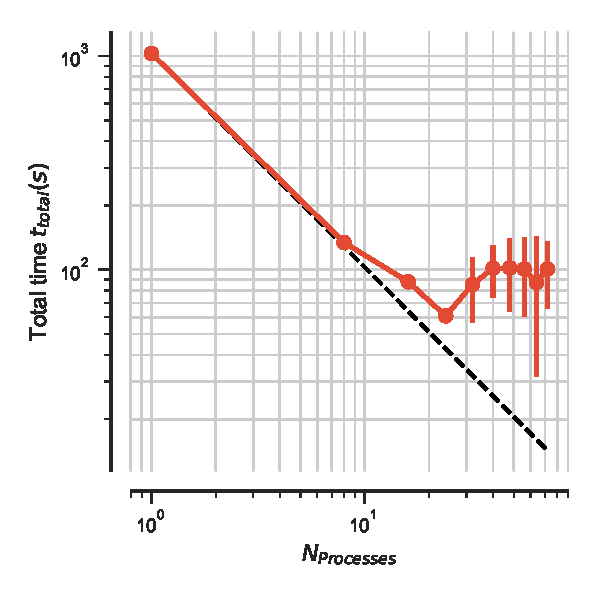
\includegraphics[width=\linewidth]{figures/main-RMSD-t_total.pdf}
  \caption{Scaling total}
  \label{fig:MPIscaling}
\end{subfigure}
\hfill
\begin{subfigure}{.4\textwidth}
  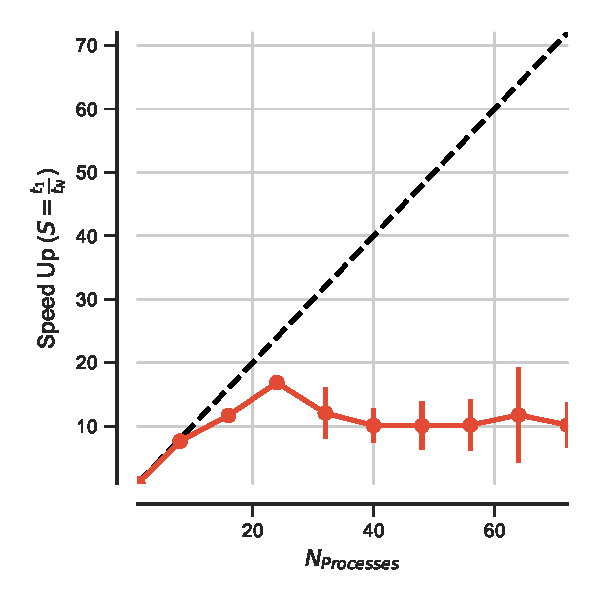
\includegraphics[width=\linewidth]{figures/main-RMSD-speed_up.pdf}
  \caption{Speed-up}
  \label{fig:MPIspeedup}
\end{subfigure}
\bigskip

\begin{subfigure}{.4\textwidth}
  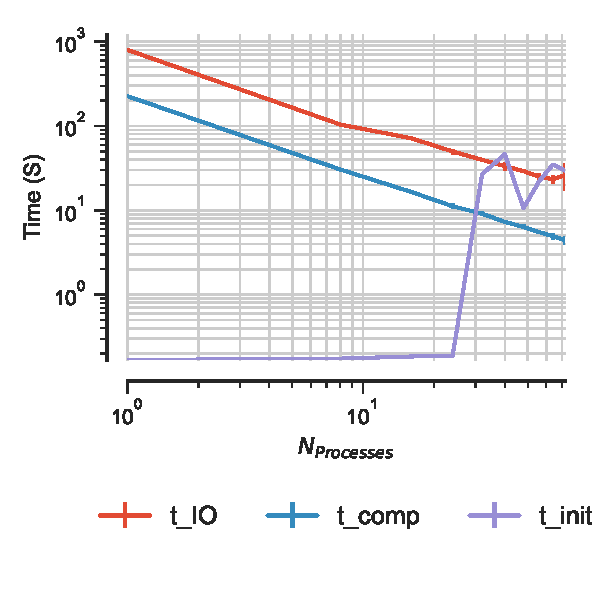
\includegraphics[width=\linewidth]{figures/main-RMSD-time_comp_IO_comparison.pdf}
\caption{\tcomp and \tIO scaling}
\label{fig:ScalingComputeIO}
\end{subfigure}
\hfill
\begin{subfigure} {.5\textwidth}
  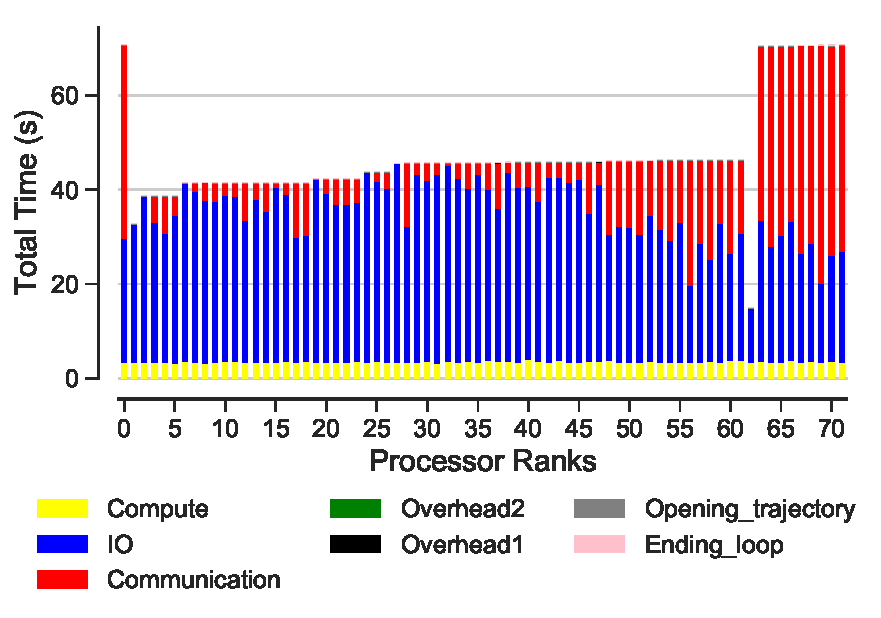
\includegraphics[width=\linewidth]{figures/main-RMSD-BarPlot-rank-comparison_72_4.pdf}
  \caption{Compute \tcomp, IO \tIO, communication \tcomm, ending the for loop $t_{end\_loop}$,
  opening the trajectory $t_{opening\_trajectory}$, and overheads $t_{Overhead1}$,  $t_{Overhead2}$ per MPI rank (as described in methods).
  This is typical data from one run of the 5 repeats}
  \label{fig:MPIranks}
\end{subfigure}

\caption{Performance of the RMSD task with MPI which is I/O-bound $\tcomp/\tIO \approx 0.3$.
Data are read from the file system (I/O included) and results are communicated back to
rank 0 (communications included). Five repeats are performed to collect statistics. The error bars show
standard deviation with respect to mean. MPI ranks 0 and 63 to 72 are stragglers, i.e., their total time 
far exceeds the mean of the majority of ranks.}
  
\obnote{This does not look like t\_comp/t\_IO = 0.3 ? looks more like 2/30 = 0.06; the next page says 4/26=0.16. Please make sure that all numbers are consistent!}
\mknote{because t\_comp/t\_IO is per frame and it is also average, what I have reported is only average.}
\label{fig:MPIwithIO}
\end{figure} 

\subsubsection*{Identification of Scalability Bottleneck}

Figure \ref{fig:ScalingComputeIO} shows the scaling of \tcomp and \tIO individulally. 
As shown, \tcomp scales very well; however, \tIO does not show good scaling beyond a single node (24 cores) and that explains why we are seeing these variations in \tIO across different ranks (Figure \ref{fig:MPIranks}). 
Considering the results in Figures \ref{fig:MPIwithIO} and \ref{fig:ScalingComputeIO}, we can conclude that communication and I/O are the root causes for stragglers. 

\subsubsection*{Hardware}
\gpnote{Are the data in figure 2 from Comet and Stampede? Why Stampede and not SuperMic, Bridges, and Comet? Those are the system you say the experimentation was done.} \mknote{the data is on Comet. We perform everything on Comet as a baseline and then make a comparison across different clusters on the final section. We do not have any data from Stampede here}
We did not discern any specific patterns that could be traced to the underlying hardware. Stragglers were observed on \emph{SDSC Comet},
\emph{TACC Stampede} and \emph{TACC Data Analytics System Wrangler} (data not shown)\gpnote{I am not sure you want to say that you do not show data. You can include them in an appendix, or provide a link to a repo with all the data and figures.}. \mknote{Ok, good idea. Will do it} There was also no clear pattern in which certain MPI
ranks would always be a straggler and we could also not trace stragglers to specific cores or nodes (or at least our data did not
reveal an obvious pattern). Therefore, the phenomenon of stragglers in the RMSD test appears to be independent from the resources.\gpnote{I would say resource independent, not hardware. Hardware opens a can of questions which is very difficult to answer with the data we have.}.\mknote{Corrected}

\subsection{Dihedral Featurization Benchmarks}
\label{DF}
We briefly tested a much larger computational workload ($t_{compute_{per-frame}}$ = 40 ms, $t_{IO_{per-frame}}$ = 0.4 ms, thus $\tcomp/\tIO \approx 100$), namely dihedral
featurization on \emph{Comet} with Infiniband and Lustre file system.

The system scales linearly and close to ideal (Figure \ref{fig:MPIscaling-dihed}, \ref{fig:MPIspeedup-dihed}, \ref{fig:ScalingComputeIO-dihed}). Although, there is communication of large
result arrays (e.g. $\approx 2GB$ with 8 processes and $\approx 0.24GB$ with 72 processes)\gpnote{Can you quantify large? Anything in terms of elements, Bytes or any other metric.}, which is costly for multiple ranks (Figure \ref{fig:comparison-t_comm-dihedral}), the speed-up curve (Eq.~\ref{eq:speedup}) in Figure \ref{fig:MPIspeedup-dihed}
demonstrates very good scaling with the number of cores (up to 72 cores on 3 nodes).  The reason is that the communication cost (for
$MPI.Gather()$-line 39 in \ref{alg:Dihedral}) decreases with increasing the number of cores because the result array size that has to be
communicated also decreases (Figure \ref{fig:comparison-t_comm-dihedral}).  Based on Figure \ref{fig:comparison-t_comm-dihedral}, communication scales fairly well
with the number of processes. This can be attributed to larger array sizes compared to the RMSD task and according to \cite{Dalcin:2011aa}
the overhead of the \package{mpi4py} package decreases as the array size to be communicated increases. The dihedral featurization workload
has larger array size for all processor sizes (per task, a time series of feature vectors of size $N_{frames} \times (213 \times 2 \times 2$) when
compared to the RMSD workload (per task a float array of length $N_{frames}$) and therefore we are hypothesizing that the higher
performance of \package{mpi4py} for larger array sizes has lead to better overall scaling. 
In addition, for higher computational workloads the competition over accessing the file is less severe as compared to lower computational workloads. 
 
\begin{figure}[ht!]
\centering
\begin{subfigure}{.4\textwidth}
  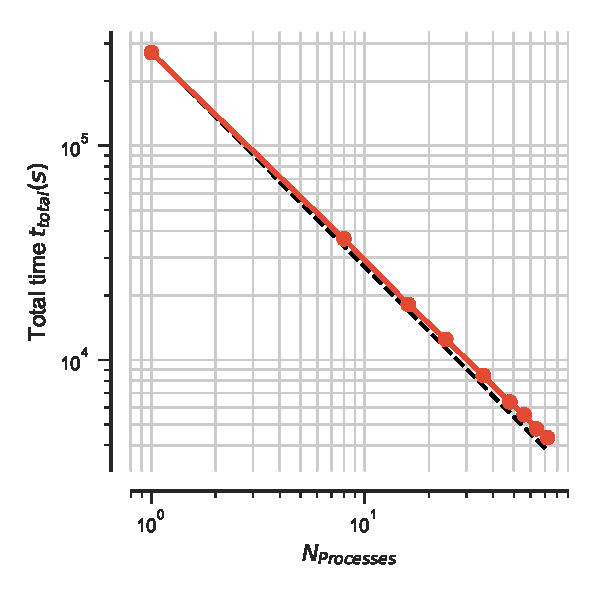
\includegraphics[width=\linewidth]{figures/main-dihedral-t_total.pdf}
  \caption{Scaling total}
  \label{fig:MPIscaling-dihed}
\end{subfigure}
\hfill
\begin{subfigure}{.4\textwidth}
  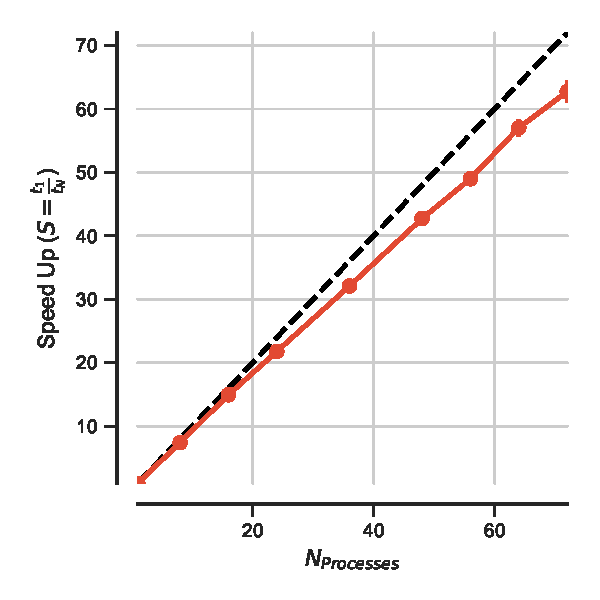
\includegraphics[width=\linewidth]{figures/main-dihedral-speed_up.pdf}
  \caption{Speed-up}
  \label{fig:MPIspeedup-dihed}
\end{subfigure}
\bigskip

\begin{subfigure} {0.4\textwidth}
  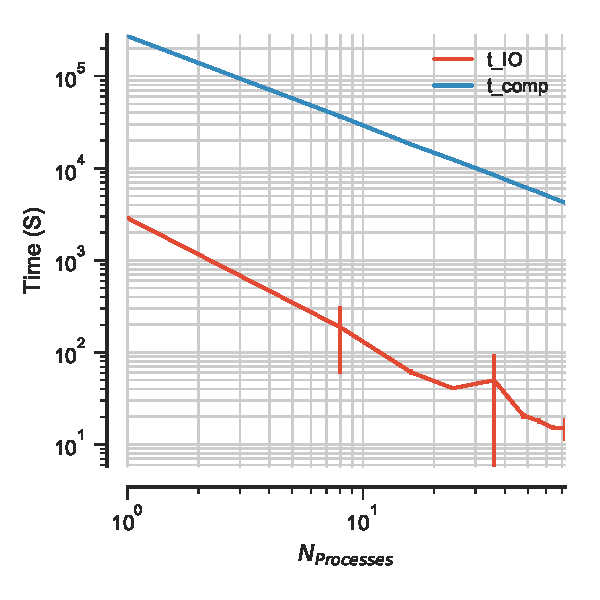
\includegraphics[width=\linewidth]{figures/main-dihed-time_comp_IO_comparison.pdf}
\caption{\tcomp and \tIO scaling}
\label{fig:ScalingComputeIO-dihed}
\end{subfigure}
\hfill
\begin{subfigure} {.5\textwidth}
  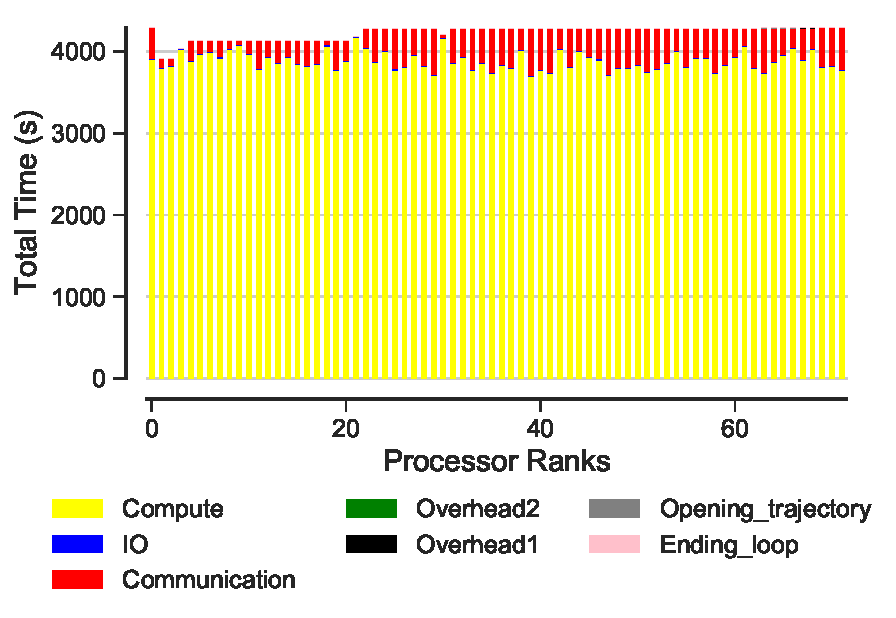
\includegraphics[width=\linewidth]{figures/main-dihedral-BarPlot-rank-comparison_72_5.pdf}
  \caption{Compute \tcomp, IO \tIO, communication \tcomm, ending the for loop $t_{end\_loop}$,
  opening the trajectory $t_{opening\_trajectory}$, and overheads $t_{Overhead1}$,  $t_{Overhead2}$ per MPI rank (as described in methods).
  This is typical data from one run of the 5 repeats}
  \label{fig:MPIranks-dihed}
\end{subfigure}

\caption{Performance for the \textbf{dihedral featurization} workload,
which is compute-bound $\tcomp/\tIO \approx 100$. Data are read from the file system (I/O included) 
and results are communicated back to rank 0 (communications included). Five repeats are performed to collect statistics. 
The error bars show standard deviation with respect to mean. No straggler is observed.} 
\label{fig:MPIwithIO-dihed}
\end{figure} 

\begin{figure}[ht!]
\begin{subfigure} {.55\textwidth}
  \centering
  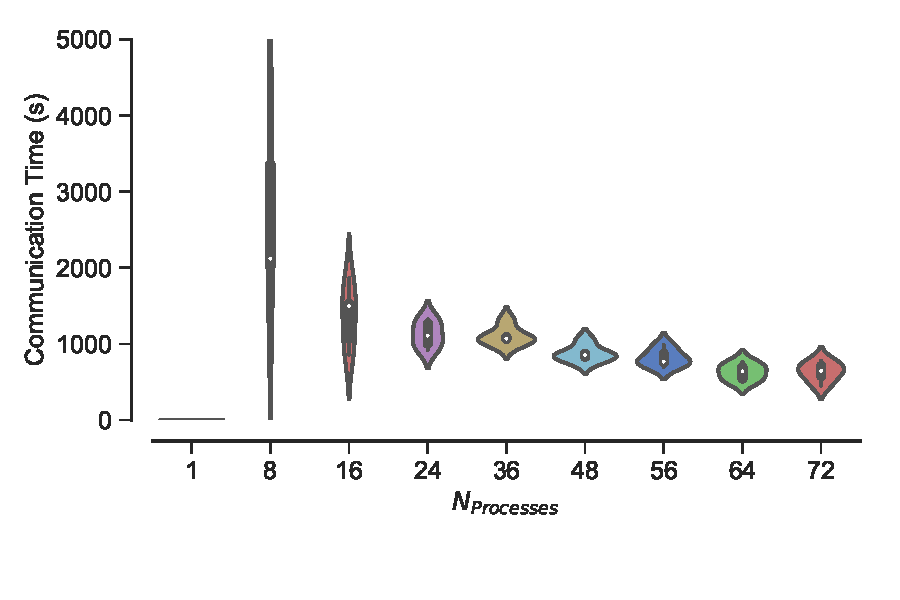
\includegraphics[width=\linewidth]{figures/ViolinPlot-Ncores-comparison-comm-dihedral.pdf}
  \caption{Communication time distribution for different number of
    processes (shown as violin plots \protect\cite{Hintze:1998tw}
    with kernel density estimates as implemented in
    \package{seaborn}); the white dot indicates the median.}
\end{subfigure}
\hfill
\begin{subfigure}{.35\textwidth}
  \centering
  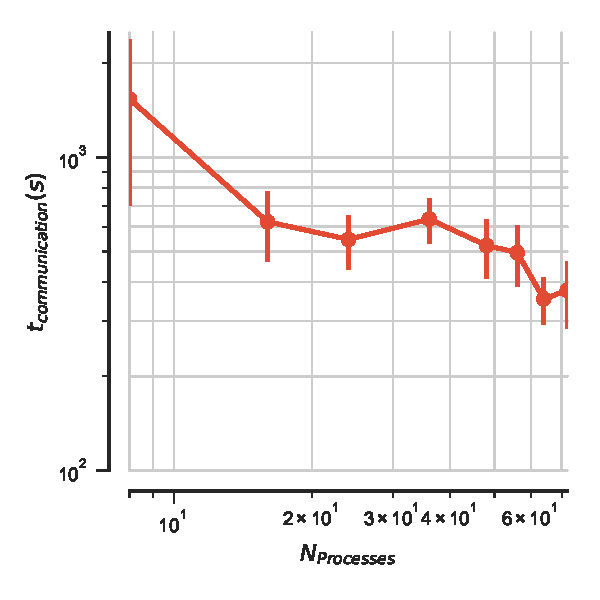
\includegraphics[width=\linewidth]{figures/t_comm_mean-dihedral.pdf}
  \caption{Scaling communcation time (mean and standard deviation)}
\end{subfigure}
\caption{Comparison of communication cost for different number of
  processes over 5 repeats for the \textbf{dihedral featurization}
  workload (with \emph{communications included}).\gpnote{I am really confused with this figure. How many GBs of data did you move and there was a delay of 1.5 hours? Was it more 10TBs? (Assuming you were able to use 20Gbps from IB $20Gbps*5000sec=10^{14}=12500000000000B=12500000000000/2^{40}TB\simeq11.6TB$)}} \mknote{with 8 processes size of the data to be communicated is 2 GB per process. But communication time is not uniform across different processes and for some processes it is in the order of 1000 for another processes is 0.86 and the other is 4 s. Thus there are stragglers due to communication but because commmunication is small with respect to compute it does not affect the performance.}
\label{fig:comparison-t_comm-dihedral}
\end{figure}

Overall, increasing the computational workload over I/O improves scaling. For large compute-bound workloads such as the dihedral
featurization task, stragglers are eliminated and nearly ideal strong scaling is achieved. 
The fact that linear scaling is possible, even with expensive communications, makes parallelization a valuable strategy to reduce
the total time to solution for large computational workloads. In a real-world application to one of our existing data sets on local
workstations with Gigabit interconnect and Network File System (NFS) (using the Dask parallel library instead of MPI), analysis time was reduced from more
than a week to a few hours (data not shown).

\subsection{Effect of \tcomp/\tIO on Performance}
\mknote{I think in addition to tcomp/tIO I need to also introduce another variable called tcomp/tcomm and In fact we can show that this is another important performance parameter. 
In fact the data with splitting without GA and parallel IO and Dihedral featurization shows that this can be another important factor as well.}

\label{bound}

The RMSD task turned out to be I/O bound, i.e.,
\begin{gather*}
  \frac{\tcomp}{\tIO} \ll 1.
\end{gather*}

and we were not able to achieve good scaling above a single node. 
However, Dihedral featurization turned out to be compute bound and we were able to achieve near ideal scaling. 
We therefore, hypothesized that decreasing the relative I/O load with respect to compute load would also reduce the stragglers. 
We therefore increased the computational load so that the work became compute bound, i.e.,

\begin{gather*}
  \frac{\tcomp}{\tIO} \gg 1.
\end{gather*}

i.e., now processes are not constantly performing I/O and instead, I/O is interleaved with longer periods of computation.
In order to artificially increase the computational load we repeated the same RMSD calculation (line 10, algorithm \ref{alg:RMSD}) 40, 70 and 100 times in a loop respectively.

\subsubsection{Increased workload (RMSD)}
The RMSD workload was artificially increased forrty-fold (``$40\times$'' ), seventy-fold (``$70\times$'' ), and hundred-fold (``$100\times$'' ) and we measured performance as before. 
These workloads correspond to \tcomp/\tIO ratio of 12, 21, 30 respectively as shown in Table \ref{tab:load-ratio}.
We performed this experiment to show the effect of $\tcomp/\tIO$ ratio on performance (Figure \ref{fig:tcomp_tIO_effect}).
On average, each rank\textsc{\char13}s workload is $N_{frames} \times \tIO $ (where $N_{frames}=N_{frames}^{total}/N$ is the
number of frames per trajectory block, i.e., the number of frames
processed by each MPI rank for $N$ processes) for I/O, and
$X \times N_{frames} \times \tcomp$ for the RMSD calculation. 
$X$ is the factor by which we increase the RMSD compute workload in our experiment.

\begin{table}[ht!]
\centering
\begin{tabular}{c c}
  \toprule
           \bfseries\thead{Workload} & \bfseries\thead{$\tcomp/\tIO$}\\
  \midrule
    RMSD $1\times$ & 0.3\\  
    RMSD $40\times$ & 12\\    
    RMSD $70\times$ & 21\\  
    RMSD $100\times$ & 30\\  
  \bottomrule
\end{tabular}
\caption[Change in load-ratio with RMSD workload]
{Change in \tcomp/\tIO ratio with change in the RMSD workload. We artificially increased the RMSD workload in order to
examine the effect of compute to I/O ratio on the performance.}
\label{tab:load-ratio}
\end{table}

As the $\tcomp/\tIO$ ratio increases, speed-up and performance improves and 
show overall better scaling than the I/O-bound workload, i.e. $1\times$ RMSD (Figure \ref{fig:S1_tcomp_tIO_effect}).
When $\tcomp/\tIO$ ratio increases, the RMSD calculation consistently scales up to larger numbers of cores ($N=56$ for $70\times$ RMSD).
Figures \ref{fig:S2_tcomp_tIO_effect} and \ref{fig:E_tcomp_tIO_effect} shows the improvment in performance more clearly.
In fact, as the $\tcomp/\tIO$ ratio increases, the values of speed-up and efficiency get closer to their ideal value for each number of processor count.  

\begin{figure}[ht!]
\centering
\begin{subfigure} {.3\textwidth}
  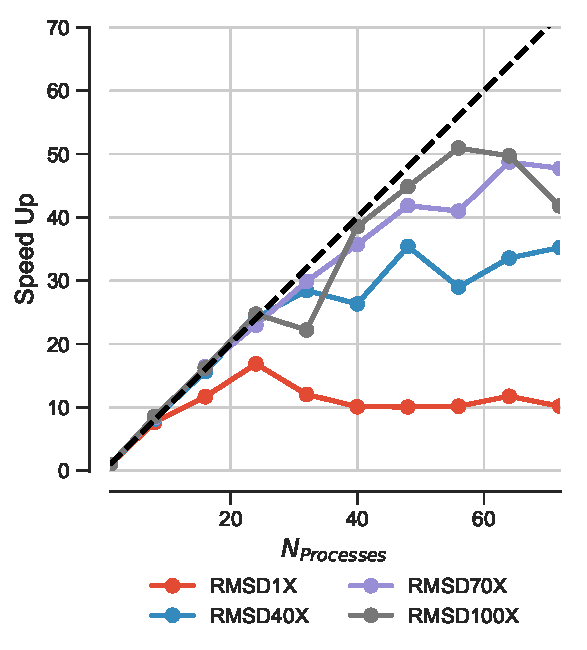
\includegraphics[width=\linewidth]{figures/Compute_to_IO_ratio_on_performance_2d_v17.pdf}
  \caption{Effect of \tcomp/\tIO on the Speed-Up}
  \label{fig:S1_tcomp_tIO_effect}
\end{subfigure}
\hfill
\begin{subfigure}{.3\textwidth}
  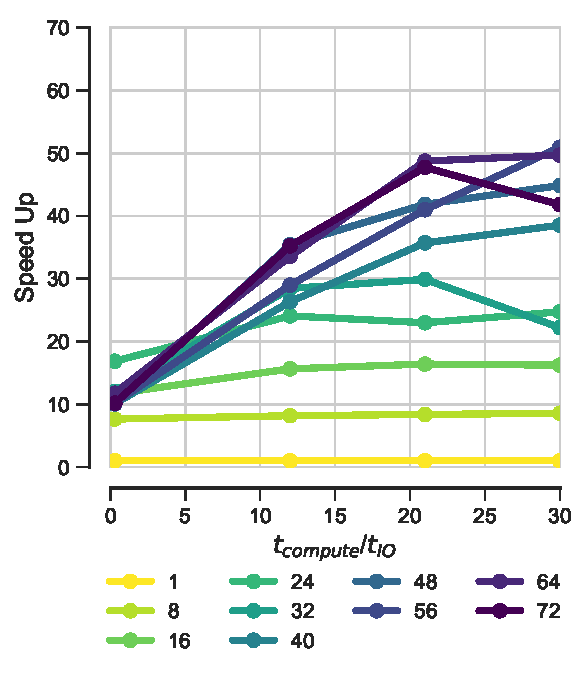
\includegraphics[width=\linewidth]{figures/Compute_to_IO_ratio_on_performance_2d_2_v17.pdf}
  \caption{Change in the Speed-Up with respect to \tcomp/\tIO for different processor counts}
  \label{fig:S2_tcomp_tIO_effect}
\end{subfigure}
\hfill
\begin{subfigure}{.3\textwidth}
  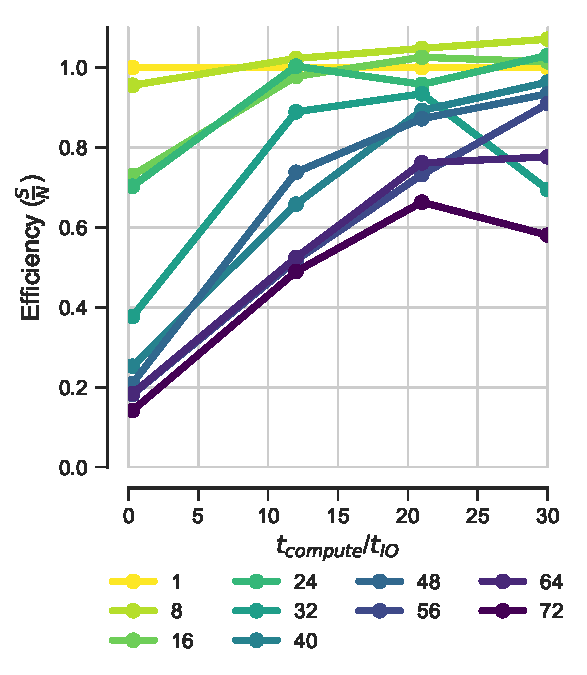
\includegraphics[width=\linewidth]{figures/Compute_to_IO_ratio_on_performance_2d_3_v17.pdf}
  \caption{Change in the efficiency with respect to \tcomp/\tIO for different processor counts}
  \label{fig:E_tcomp_tIO_effect}
\end{subfigure}
%
\caption{Performance change of the RMSD task with MPI with different $\tcomp/\tIO$ ratios. We tested performance for $\tcomp/\tIO$ ratios of 0.3, 12, 21, 30
which correspond to $1\times$ RMSD, $40\times$ RMSD, $70\times$ RMSD, and $100\times$ RMSD respectively (communication is included)}
\label{fig:tcomp_tIO_effect}
\end{figure}

Even for moderately compute-bound workloads such
as the $40\times$ and $70\times$ RMSD tasks, increasing the computational workload over I/O reduced the impact of stragglers even
though they still contribute to large variations in timing across different ranks and thus to somewhat erratic scaling.\gpnote{What is erratic scaling? Can you quantify it?}

Given the results for Dihedral featurization and RMSD algorithms (Algorithms \ref{alg:Dihedral}, and \ref{alg:RMSD}) and $X\times$ RMSD (Figure \ref{fig:tcomp_tIO_effect})
we hypothesize that MPI competes with Lustre on the same network interface, which would explain why communication appears to
be primarily a problem in the presence of I/O when \tcomp/\tIO is small.
In fact, decreasing the I/O load relative to the compute load should open up the network for communication. 

\subsection{Communication Cost and Application of Global Array}
\label{Global-Array}
As discussed in the previous sections, Figure \ref{fig:MPIranks}, for small \tcomp/\tIO communication acts as the scalability bottleneck. 
In fact, when the processes communicate result arrays back to the master process (rank 0), some processes take much longer as compared to other processes. 
Now we want to know what strategies can be used to avoid communication cost. 

We used global array instead of collective communication in MPI and examined the change in the performance. 
In global array, we define one large RMSD array, and each MPI rank updates its associated block in the global RMSD array using $ga\_put$. 
At the end, when all the processes exit \texttt{block\_rmsd()} function and update their local block in the global array, rank 0 will access the whole global array using $ga\_access$.
In fact, in global arrays the time for communication is $t_{ga\_put}+t_{ga\_access}$.
Given the speed up plots (Figure \ref{fig:MPIspeedup-ga4py}) and total time scaling (Figure \ref{fig:MPIscaling-ga4py}) global array improves strong scaling performance.
Although communication time has significantly decreased using global array (compare Figure \ref{fig:MPIranks-ga4py} to Figure \ref{fig:MPIranks}),
the existing variation in the dominant I/O part of the calculation plus two delayed MPI ranks due to the delay in opening the trajectory would still prevent ideal scaling (Figure \ref{fig:ScalingComputeIO-ga4py}).
This figure shows only one repeat out of 5 we performed for our benchmark study. 
Opening the trajectory was not a problem in other repeats.
In fact, although communications were performed using global arrays, scaling is still far from ideal as a result of slow processes due to I/O variation and the delay in opening the trajectory.
\obnote{In Fig 8c it is the trajectory opening step that creates stragglers. This was not a problem before. Is this now ALWAYS the problem when using GA? Needs to be discussed. }
\mknote{no only happened in one repeat. Does not seem to me to be a problem with GA}
These slow processes take about 50~s, which are slower than the mean execution time of all ranks, i.e. 17~s. 

\begin{figure}[ht!]
\centering
\begin{subfigure}{.4\textwidth}
  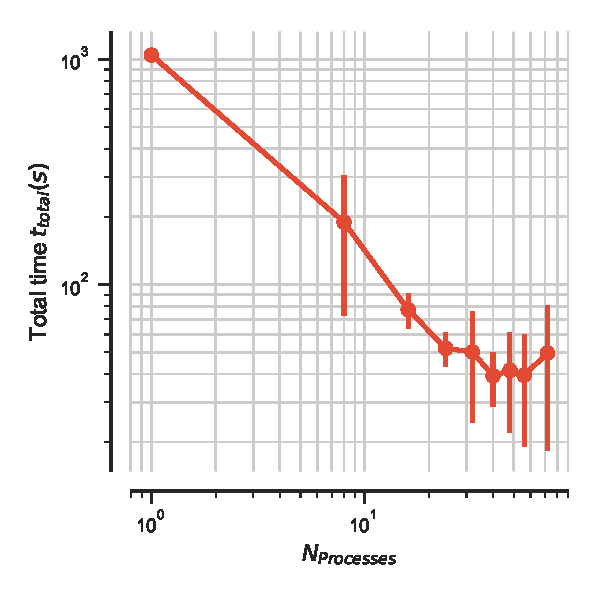
\includegraphics[width=\linewidth]{figures/RMSD-ga4py-t_total.pdf}
  \caption{Scaling total}
  \label{fig:MPIscaling-ga4py}
\end{subfigure}
\hfill
\begin{subfigure}{.4\textwidth}
  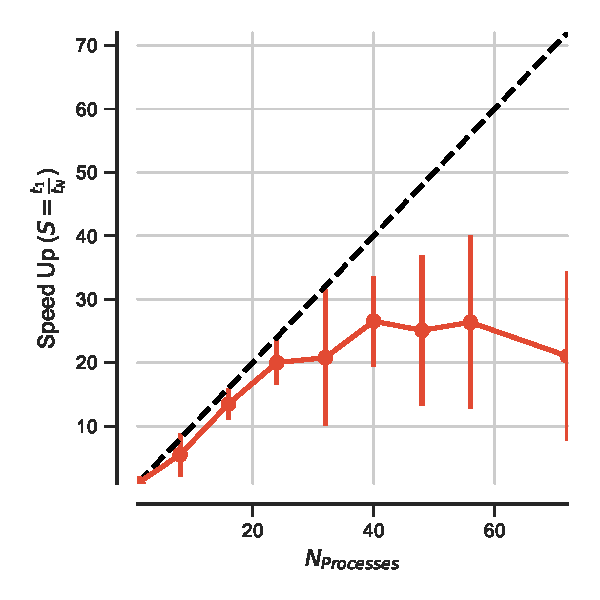
\includegraphics[width=\linewidth]{figures/RMSD-ga4py-speed_up.pdf}
  \caption{Speed-up}
  \label{fig:MPIspeedup-ga4py}
\end{subfigure}
\bigskip

\begin{subfigure}{.4\textwidth}
  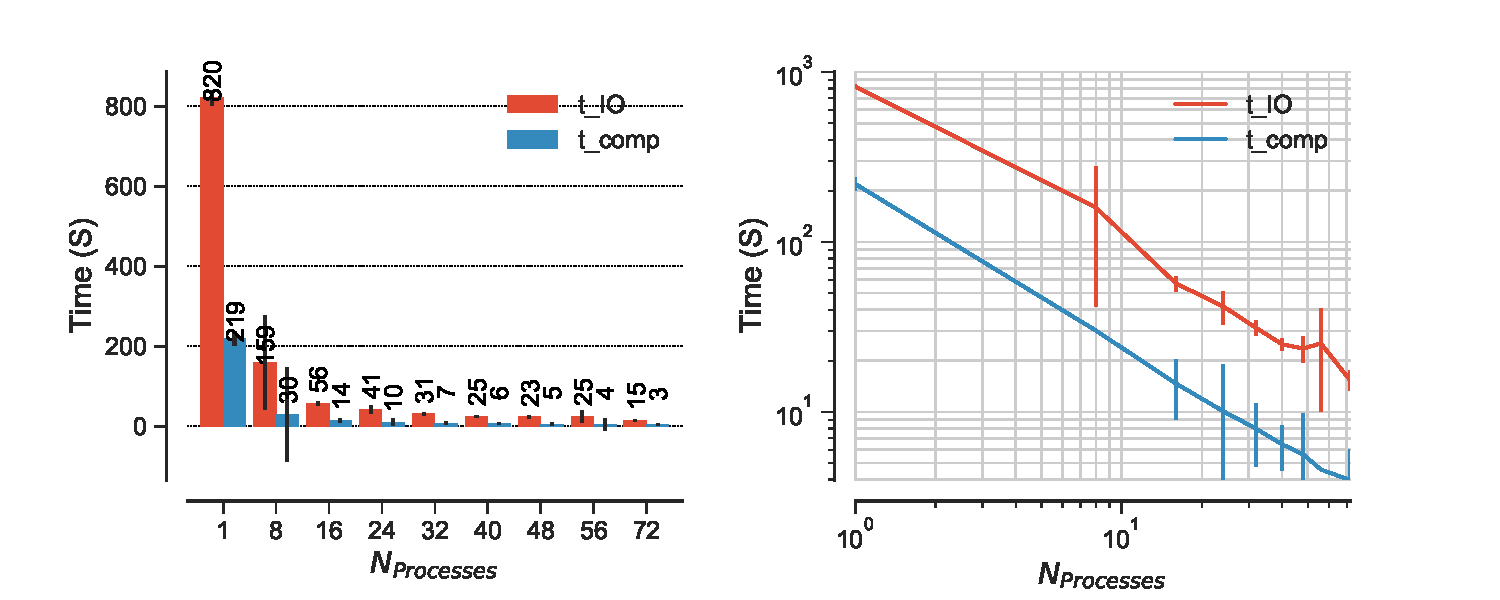
\includegraphics[width=\linewidth]{figures/RMSD-ga4py-time_IO_comparison.pdf}
\caption{\tcomp and \tIO scaling}
\label{fig:ScalingComputeIO-ga4py}
\end{subfigure}
\hfill
\begin{subfigure} {.5\textwidth}
  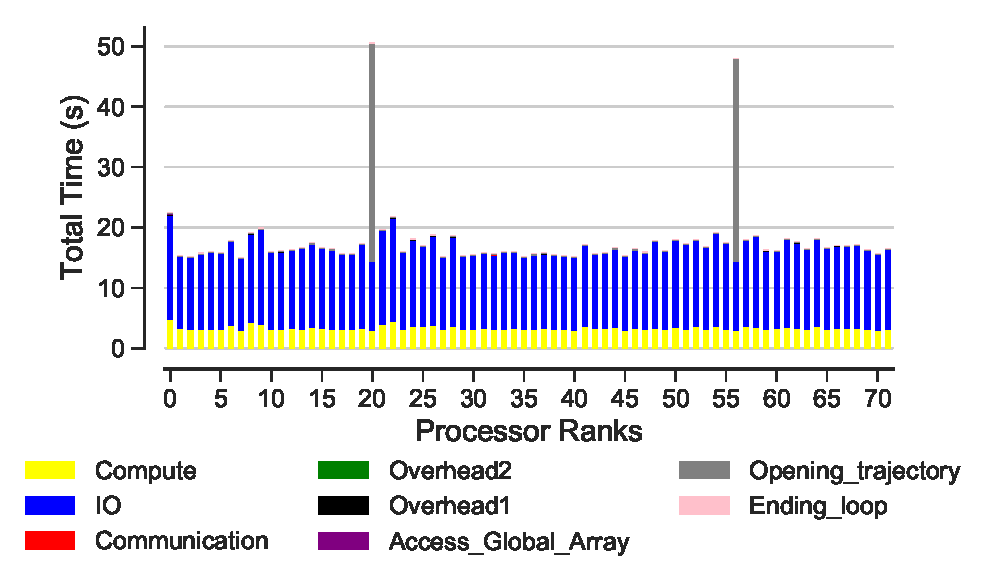
\includegraphics[width=\linewidth]{figures/RMSD-ga4py-BarPlot-rank-comparison_72_1.pdf}
  \caption{Compute \tcomp, IO \tIO, communication \tcomm , ending the for loop $t_{end\_loop}$,
  opening the trajectory $t_{opening\_trajectory}$, and overheads $t_{Overhead1}$,  $t_{Overhead2}$ per MPI rank (as described in methods).
  This is typical data from one run of the 5 repeats}
  \label{fig:MPIranks-ga4py}
\end{subfigure}

\caption{Performance of the RMSD task with MPI using global array ($\tcomp/\tIO \approx 0.3$).
Data are read from the file system (I/O included). All ranks update the global array and rank 0 accesses the whole RMSD array.
Five repeats are performed to collect statistics. The error bars show standard deviation with respect to mean. 
MPI ranks 20 and 56 are stragglers, i.e., their total time far exceeds the mean of the majority of ranks.}
\label{fig:MPIwithIO-ga4py}
\end{figure}

\subsection{I/O Cost}
\label{I/O}
We showed previously that the I/O system can have a large effect on the parallel performance of the RMSD task \cite{Khoshlessan:2017ab},
especially because the average time to perform the computation \tcomp (about 0.09 ms) is about three times smaller than the I/O time \tIO (about 0.3 ms) (Figures \ref{fig:ScalingComputeIO} and \ref{fig:MPIwithIO}). 
In fact, poor I/O performance is responsible for the stragglers, and the question is ``are stragglers waiting for file access?". 
Due to the large file size and memory limit, processes are not able to load the whole trajectory into memory at once and as a result each process is only allowed to load one frame into memory at a time.
The test trajectory has about $2,512,200$ frames in total and as a result there will be $2,512,200$ file access requests. 
Thus, when the compute time is small with respect to I/O, then I/O can be a major issue as we also see in our results (Figures \ref{fig:ScalingComputeIO} and \ref{fig:MPIwithIO}).    
Read throughput might be limited by the available bandwidth on the Infini-band network interface that serves the Lustre file system and access to files might be throttled.
We show that depending on the cluster and its capabilities the throughput might become a problem for achieving good performance and we also show ways to overcome this problem and improve performance.
In fact, we need to come up with ways and strategies to avoid the competition over file access across different ranks when \tcomp/\tIO ratio is small.
To this aim, we experimented two different ways for reducing I/O cost and examined their effect on the performance.
These two ways include: Splitting the trajectory file into as many segments as number of processes and MPI-based Parallel HDF5.
We discuss these two approaches in detail in the following sections.

\subsubsection{Splitting the Trajectories}
\label{Splitting}
In all the previous benchmarks all processes were using a shared trajectory file.
In order to test our hypothesis that \emph{I/O and communication compete over the network resources with small \tcomp/\tIO ratio}, we splitted our trajectory file into as many trajectory segments as the number of processes.
This means that if we have $N$ processes, the trajectory file is splitted into $N$ segments and each segment will have $N_{b}$ frames in it. 
Through this approach, each process will have access to its own segment and there will be no competition over file accesses. 
For reference, the necessary time for splitting the trajectory file is given in \ref{sec:splitting-timing}.

\subsubsection*{Performance without Global Array}
We ran a benchmark up to 8 nodes (192 cores) and, we observed rather better scaling behavior with efficiencies above 0.6 (Figure \ref{fig:MPIscaling-split} and \ref{fig:MPIspeedup-split}) and the delay time for stragglers has also reduced from 65s to about 23s (Compare Figure \ref{fig:MPIranks-split} to  \ref{fig:MPIranks}). 
However, the scaling is still far from ideal due to the communication. 
Although the delay due to communication is much smaller as compared to RMSD with a shared trajectory file (Compare Figure \ref{fig:MPIranks-split} to Figure \ref{fig:MPIranks}), it is still delaying several processes and as a result leads to longer job completion time (Figure \ref{fig:MPIranks-split}). 
These delayed tasks impact performance as well and hence the speed-up is not still close to ideal scaling (Figure \ref{fig:MPIspeedup-split}).

\begin{figure}[ht!]
\centering
\begin{subfigure}{.4\textwidth}
  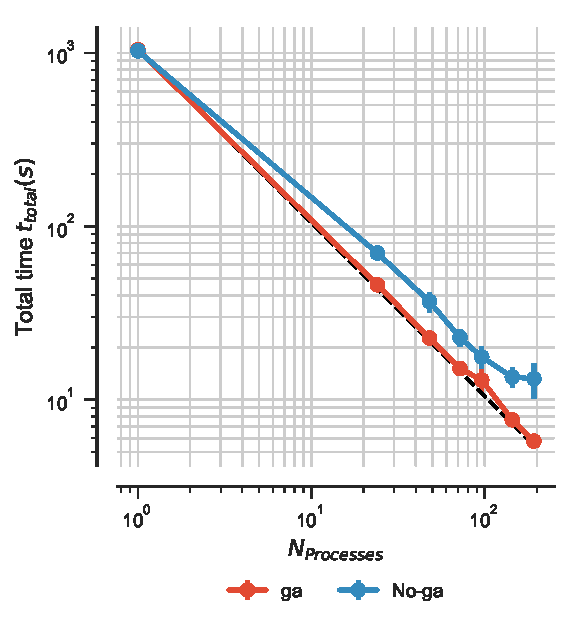
\includegraphics[width=\linewidth]{figures/Comparison_tot_time_traj_splitting.pdf}
  \caption{Scaling total}
  \label{fig:MPIscaling-split}
\end{subfigure}
\hfill
\begin{subfigure}{.4\textwidth}
  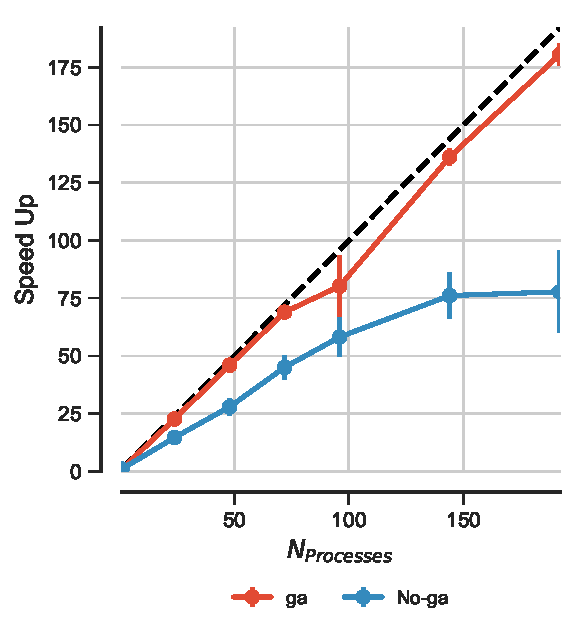
\includegraphics[width=\linewidth]{figures/Comparison_Speed_UP_traj_splitting.pdf}
  \caption{Speed-up}
  \label{fig:MPIspeedup-split}
\end{subfigure}
\bigskip

\begin{subfigure} {.5\textwidth}
  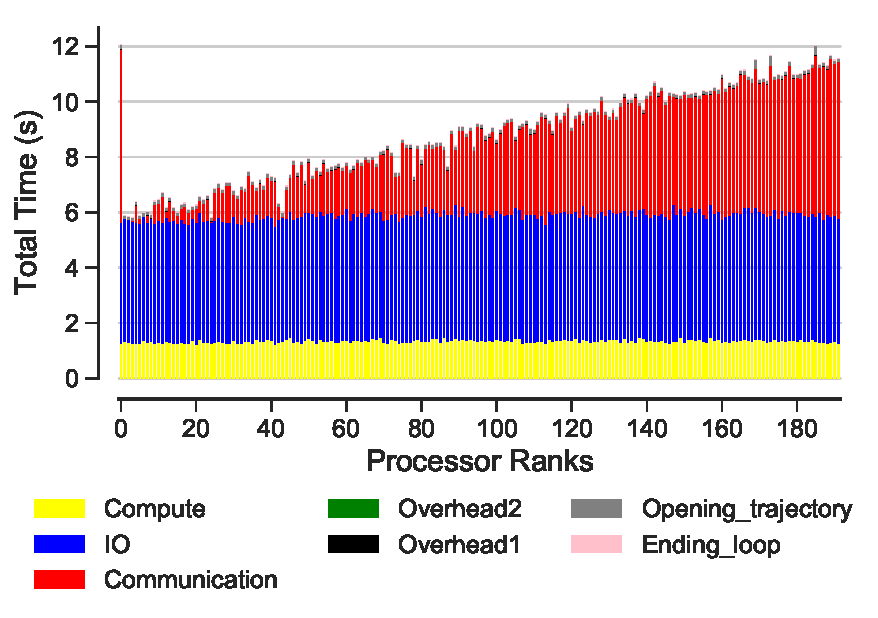
\includegraphics[width=\linewidth]{figures/split-BarPlot-rank-comparison_192_5.pdf}
   \caption{Examples of timing per MPI rank without global array}
  \label{fig:MPIranks-split}
\end{subfigure}
\hfill
\begin{subfigure} {.5\textwidth}
  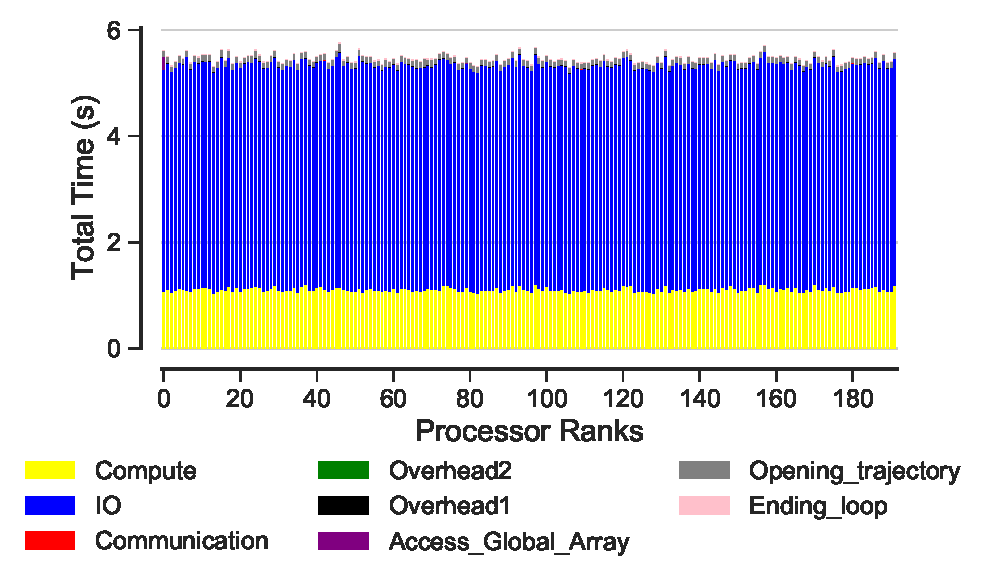
\includegraphics[width=\linewidth]{figures/split-ga-BarPlot-rank-comparison_192_5.pdf}
  \caption{Examples of timing per MPI rank using global array}
  \label{fig:MPIranks-split-ga}
\end{subfigure}

\caption{Comparison on the performance of the RMSD task with MPI when the trajectories are splitted using global array and without global array ($\tcomp/\tIO \approx 0.3$).
Data are read from the file system (I/O included). In case of global array, all ranks update the global array ($ga_{put}$) and rank 0 accesses the whole RMSD array through the global memory address ($ga_{get}$).}
\label{fig:MPIwithIO-split}
\obnote{The compute/IO ratio is about 1:4 judging from the graph, i.e., ~0.25 ? or did you calculate the ratio for the serial version?}
\mknote{Yes, this is based on serial version}
\end{figure}

\begin{figure}[ht!]
\centering
  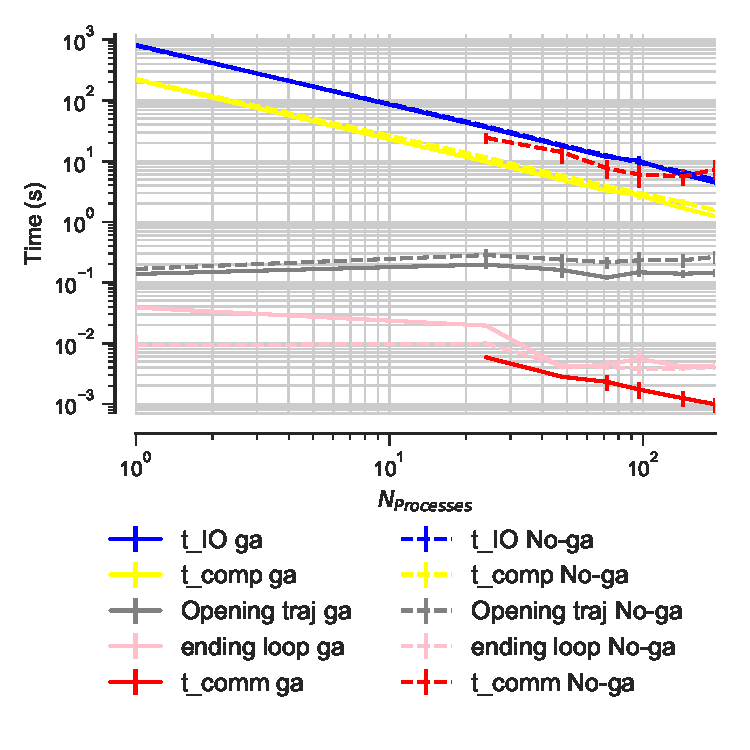
\includegraphics[width=0.4\linewidth]{figures/Comparison_IO_compute_scaling_traj_splitting.pdf}
\caption{Comparison on the scaling of the \tcomp and \tIO of the RMSD task when the trajectories are splitted with global array and without global array.}
\label{fig:ScalingComputeIO-split}
\end{figure}

\subsubsection*{Performance using Global Array}
\gpnote{This is very confusing. In a previous paragraph you say that GA passes data over the IB network. Here you say there is no congestion? Don't they, MPI communication, MPI I/O, and GA communication, use the same network? Also, I do not think you have the data to support that clearly, unless you know how many Bytes are moved around, how many packets and their type. If that is the case include it. Or are you using the Local filesystem on the nodes and IO has nothing to do with the IB?}
Previously, we showed that global array significantly reduces the communication cost (Section \ref{Global-Array}). 
We want to see how the performance looks like if we split our trajectory file and take advantage of global array as well.
Again, we ran our benchmark up to 8 nodes (192 cores) and, we observed near ideal scaling behavior with efficiencies above 0.9 (Figure \ref{fig:MPIscaling-split} and \ref{fig:MPIspeedup-split}) with no straggler tasks (Figure \ref{fig:MPIranks-split-ga}).  
The present results show that contention for a file impacts the performance. 
The initial results with splitting the trajectory file suggests that there is in fact an effect, which possibly also interferes with the communications when $\tcomp/\tIO \ll 1$ (i.e. with a I/O bound workload).

\subsubsection{Chain-Reader}

\subsubsection{MPI-based Parallel HDF5}
\label{HDF5}
Another approach we examined to improve I/O scaling is MPI-based Parallel HDF5. 
We converted our XTC trajectory file into HDF5 format so that we can test the performance of parallel IO with HDF5 file format.
The time it took to convert our XTC file with $2,512,200$ frames into HDF5 format was about $5400~s$ in our local resources with network file system (NFS).
Again, we ran our benchmark up to 8 nodes (192 cores) and, we observed near ideal scaling behavior with efficiencies above 0.8 (Figure \ref{fig:MPIscaling-hdf5} and \ref{fig:MPIspeedup-hdf5}) with no straggler tasks (Figure \ref{fig:MPIranks-hdf5}).  
When we split our trajectory, scaling is better as compared to that of parallel I/O (Compare Figure \ref{fig:MPIspeedup-hdf5} to Figure \ref{fig:MPIspeedup-split}). 
However, both methods scale very well up to 8 nodes and have comparable performance.  

\begin{figure}[ht!]
\centering
\begin{subfigure}{.4\textwidth}
  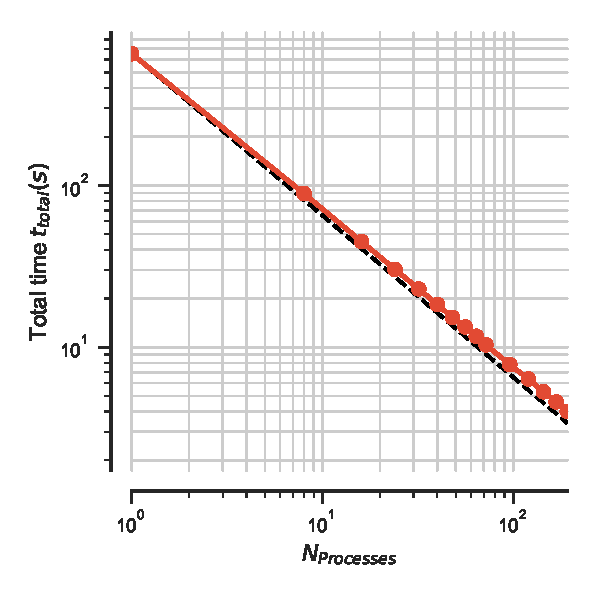
\includegraphics[width=\linewidth]{figures/hdf5-t_total.pdf}
  \caption{Scaling total}
  \label{fig:MPIscaling-hdf5}
\end{subfigure}
\hfill
\begin{subfigure}{.4\textwidth}
  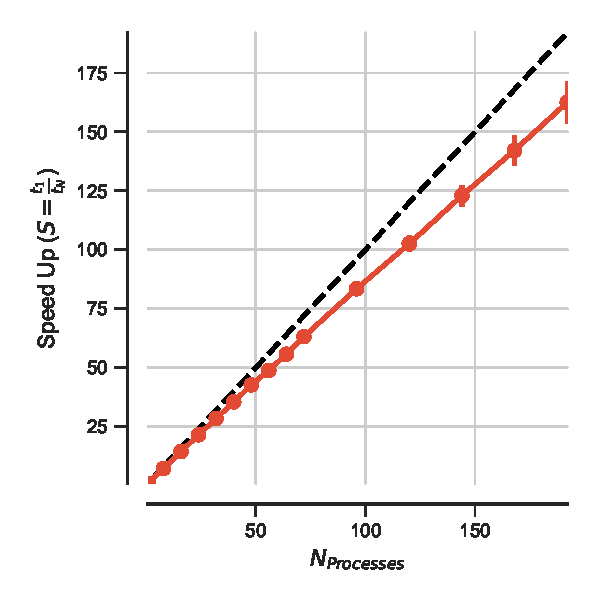
\includegraphics[width=\linewidth]{figures/hdf5-speed_up.pdf}
  \caption{Speed-up}
  \label{fig:MPIspeedup-hdf5}
\end{subfigure}
\bigskip

\begin{subfigure}{.4\textwidth}
\centering
  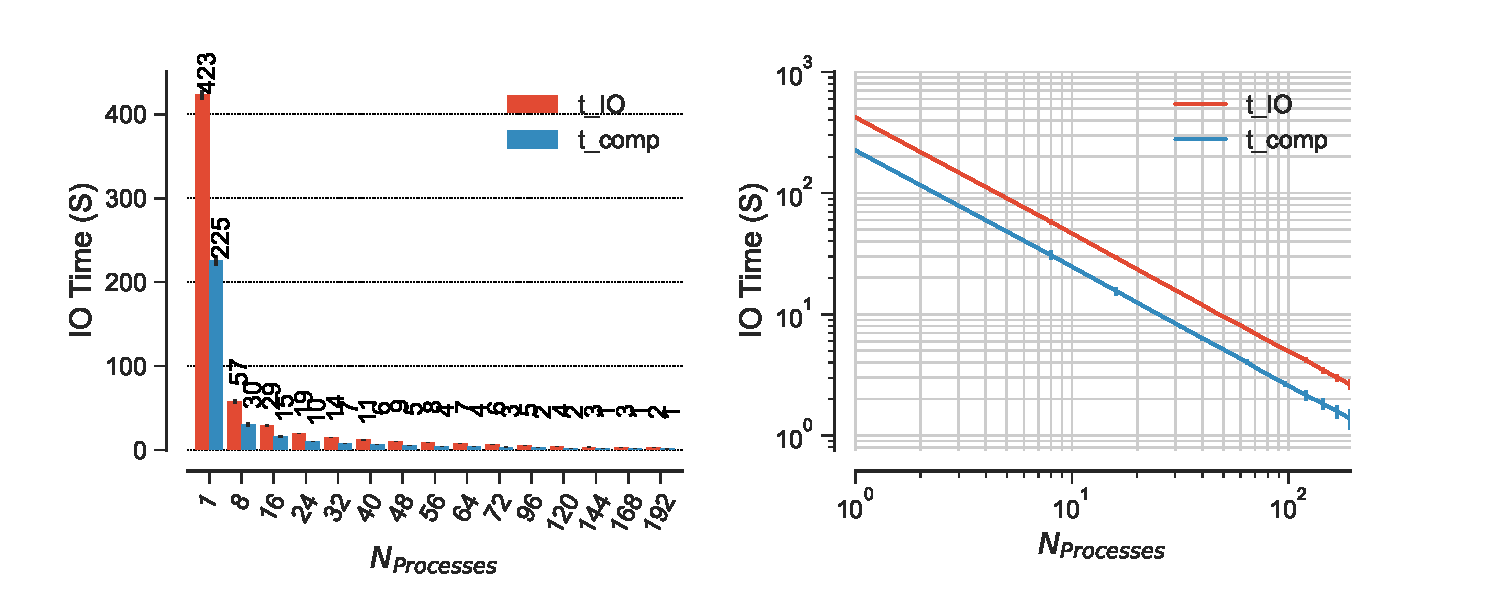
\includegraphics[width=\linewidth]{figures/hdf5-time_IO_comparison.pdf}
\caption{\tcomp and \tIO scaling}
\label{fig:ScalingComputeIO-hdf5}
\end{subfigure}
\hfill
\begin{subfigure} {.5\textwidth}
  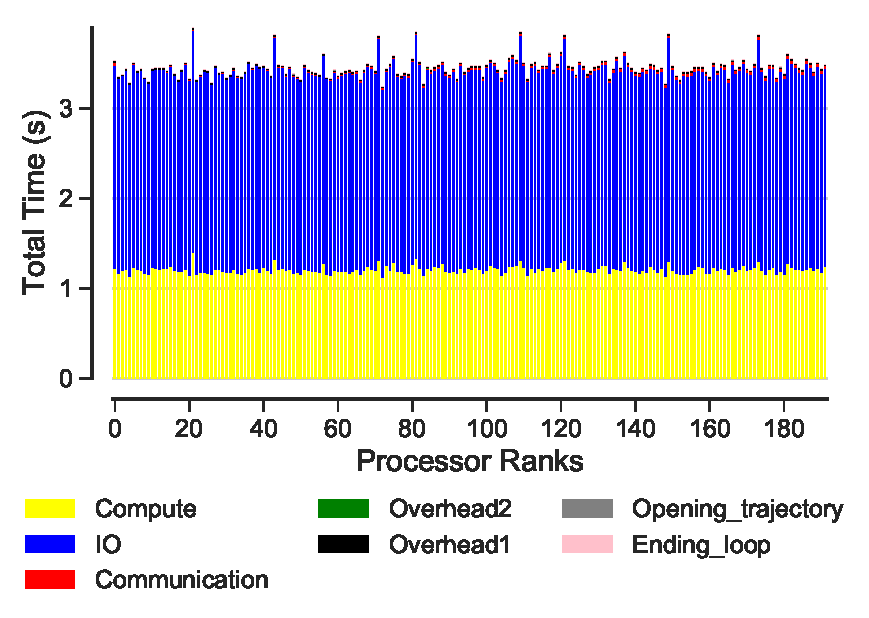
\includegraphics[width=\linewidth]{figures/hdf5-BarPlot-rank-comparison_192_4.pdf}
  \caption{Compute \tcomp, IO \tIO, communication \tcomm , ending the for loop $t_{end\_loop}$,
  opening the trajectory $t_{opening\_trajectory}$, and overheads $t_{Overhead1}$,  $t_{Overhead2}$ per MPI rank (as described in methods).}
  \label{fig:MPIranks-hdf5}
\end{subfigure}
%
\caption{Performance of the RMSD task with MPI-based parallel HDF5 ($\tcomp/\tIO \approx 0.3$).
Data are read from the file system from a shared HDF5 file instead of XTC format (Independent I/O).}
\label{fig:MPIwithIO-hdf5}
\end{figure}


\section{Performance Comparison of the RMSD task on different clusters}
\label{sec:clusters}
In this section we try to compare the performance of RMSD task on different HPC resources to examine the robustness of the methods we used for our performance study.
HPC resources used for this purpose and their system configuration are given in Table \ref{tab:sys-config}.
We perform these comparisons for several cases discussed previously. 
These cases include: Splitting the trajectories with collective communications in MPI, Splitting the trajectories with global array for communications, and MPI-based Parallel HDF5.

\subsection{Splitting the Trajectories}
Figure \ref{fig:MPI-splitting-clusters} shows how RMSD task scales with the increase in the number of cores on different HPC resources.  
When we split the trajectories the scaling follows the same pattern on both Comet and SuperMIC with global array and without global array.
Both Comet and SuperMIC scales very well using Global array. 
RMSD task still scales on both clusters without global array; however, scaling is far from ideal scaling due to the communication cost (Refer to section \ref{Splitting} and Figure \ref{fig:MPIranks-split}). 
Overal, the scaling of the RMSD task is better on SuperMIC and the performance gap increases as we increase the number of cores.
This is expected for the following reasons:
First, CPU speed on SuperMIC is 2.8 GHz vs 2.5 GHz on Comet. This is $\approx 12\%$ performance difference in favor of SuperMIC\gpnote{This type of comparing may have been correct assuming you used only 20 cores on Comet, 10 from each processor. But all of them were used, right?}. \mknote{Yes, all the cores are used but I do not understand why you say when all core numbers are used this type of comparison is not correct.}
Second, for the same network speed the number of cores per node on SuperMIC (20 cores per node) is smaller than Comet (24 cores per node). 
Therefore, access to memory per core should be factor of $12/10 \approx 20\%$ faster on SuperMIC\gpnote{Memory access performance is not measured be the number of cores accessing the memory only. First, SuperMic has DDR3, and Comet has DDR4. Just that shows us that Comet memory is better. We do not have data as memory read/write times, memory organization and architecture, that is every memory address how many data can it hold? Any information on memory throughput? I would never do this type of arithmetic to compare CPUs and memory.}\mknote{I agree with you. But do you have any suggestion on how we should discuss these differences?}
\gpnote{Also, I am not sure whether GA support direct memory access from the network card or not. If you have a reference that says so, please cite it here, otherwise I would remove the argument}.
\mknote{What is direct memory access from the network card? Why does it matter?}

\begin{figure}[ht!]
\centering
\begin{subfigure}{.4\textwidth}
  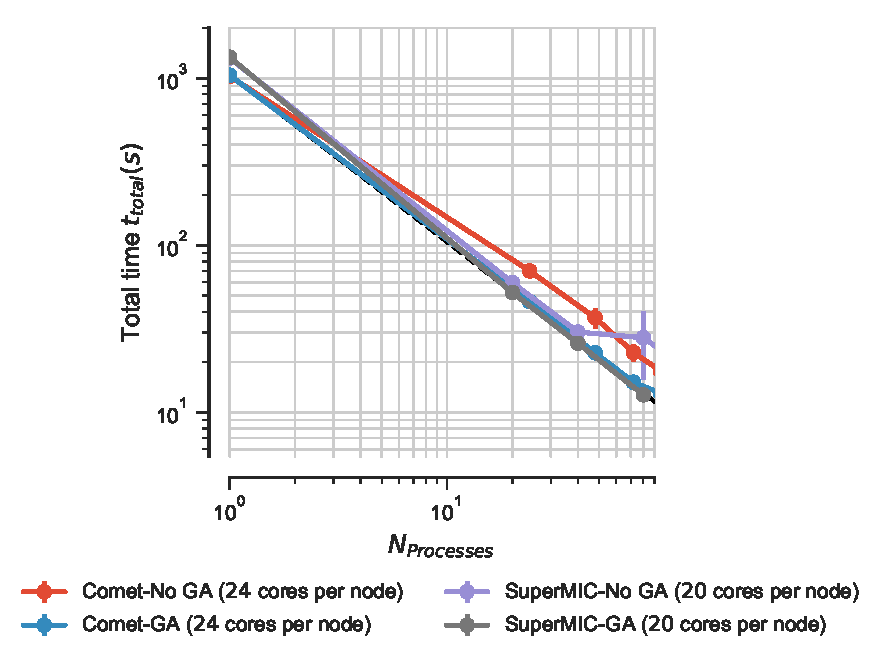
\includegraphics[width=\linewidth]{figures/Comparison_t-tot-clusters_Splitting.pdf}
  \caption{Scaling total}
  \label{fig:MPIscaling-clusters-splitting}
\end{subfigure}
\hfill
\begin{subfigure}{.4\textwidth}
  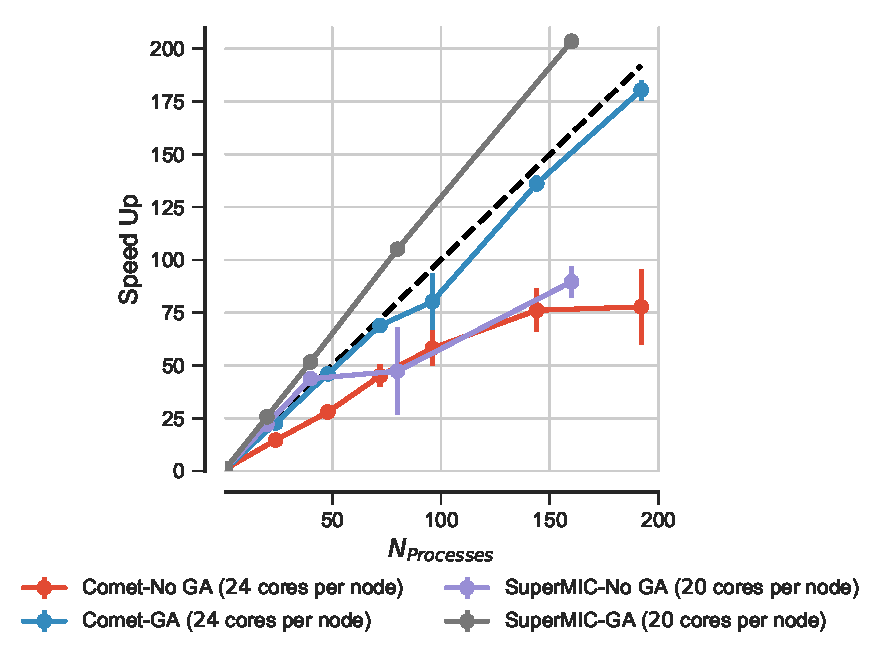
\includegraphics[width=\linewidth]{figures/Comparison_speed-up-clusters_Splitting.pdf}
  \caption{Speed-up}
  \label{fig:MPIspeedup-clusters-splitting}
\end{subfigure}
\bigskip

\begin{subfigure} {.8\textwidth}
  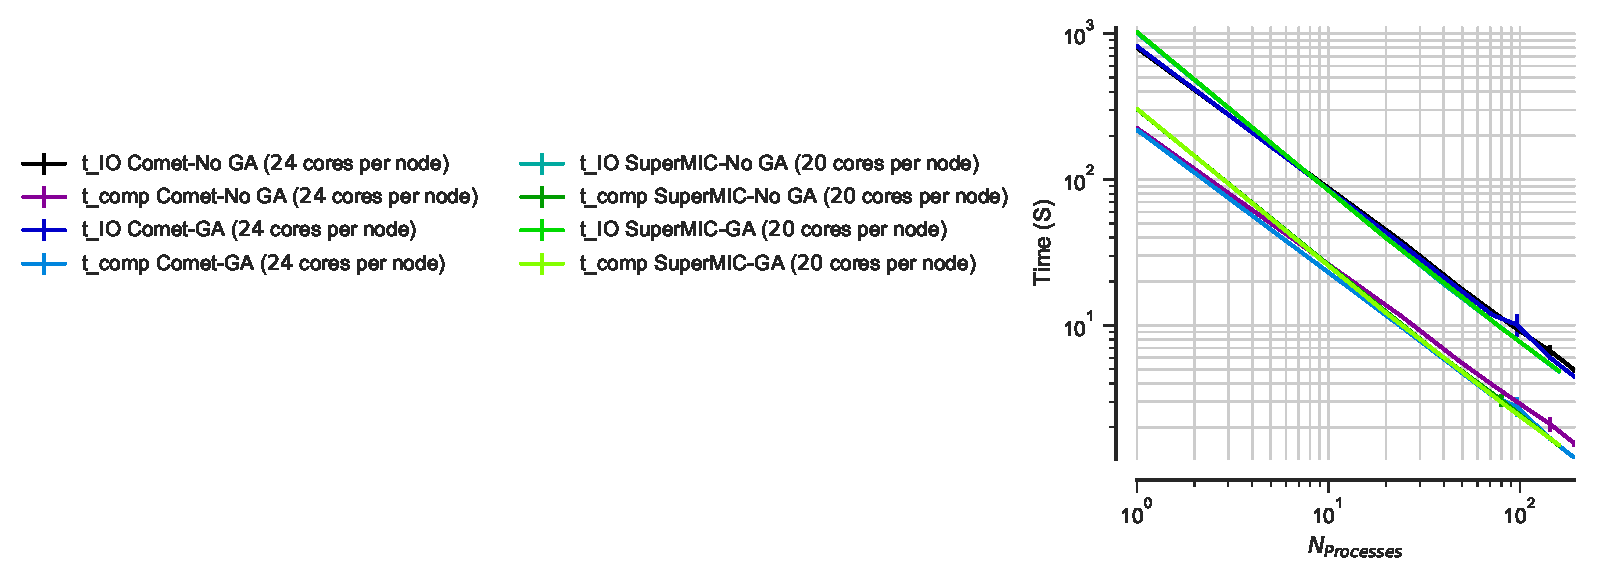
\includegraphics[width=\linewidth]{figures/Clusters_IO_compute_scaling_splitting.pdf}
  \caption{Scaling of the \tcomp and \tIO of the RMSD task with MPI when the trajectories are splitted using global array and without global array.}
  \label{fig:compute-IO-scaling-clusters-splitting}
\end{subfigure}
%
\caption{Comparison of the performance of the RMSD task with MPI ($\tcomp/\tIO \approx 0.3$) when the trajectories are splitted using global 
array and without global array across different clusters (SDSC Comet, SuperMIC). Data are read from the file system (I/O included).
In case of global array, all ranks update the global array ($ga_{put}$) and rank 0 accesses the whole RMSD array through the global memory address ($ga_{get}$).
Five repeats are performed to collect statistics. The error bars show standard deviation with respect to mean. }
\label{fig:MPI-splitting-clusters}
\end{figure} 

\subsection{MPI-based Parallel HDF5}
\gpnote{Same as above}
Figure \ref{fig:MPIwithIO-clusters} shows how RMSD task scales with the increase in the number of cores on different HPC resources using MPI-based parallel HDF5.  
The scaling follows the same pattern on both Comet and SuperMIC. 
Both Comet and SuperMIC scales very well.
Overal, the scaling of the RMSD task is better on SuperMIC for the reasons that discussed above.
Bridge performance is different from Comet and SuperMIC.
Bridge has 28 cores per compute node and when we use all cores for our calculations there is no scaling.
However, decreasing the number of cores per node and having uniform workload distributions across all nodes can lead to significant improvements in the scaling as shown in Figure \ref{fig:MPIwithIO-clusters}.
The reason for performance difference between Comet and Bridges can be explained as below:
First, CPU speed on Bridges is 2.3 GHz vs 2.5 GHz on Comet. This is $\approx 8.6\%$ performance difference in favor of Comet. 
Second, for the same network speed the number of cores per node on Bridge (28 cores per node) is larger than Comet (24 cores per node). 
Therefore, access to memory per core should be factor of $14/12 \approx 16\%$ faster on Comet.
The memory access effect on the timing distribution across different rank is shown for one run of the 5 repeats (Figure \ref{fig:MPIwithIO-clusters-rank}).
Based on Figure \ref{fig:MPIwithIO-clusters-rank} the I/O time distribution is pretty small and uniform across all ranks on Comet and SuperMIC (Figures \ref{fig:hdf5-SuperMIC} \& \ref{fig:MPIranks-hdf5}).
However, on Bridges the I/O time is on average about two and a half times larger and the I/O time distribution is also erratic across different ranks (Figure \ref{fig:hdf5-bridge}).  

\begin{figure}[ht!]
\centering
\begin{subfigure}{.4\textwidth}
  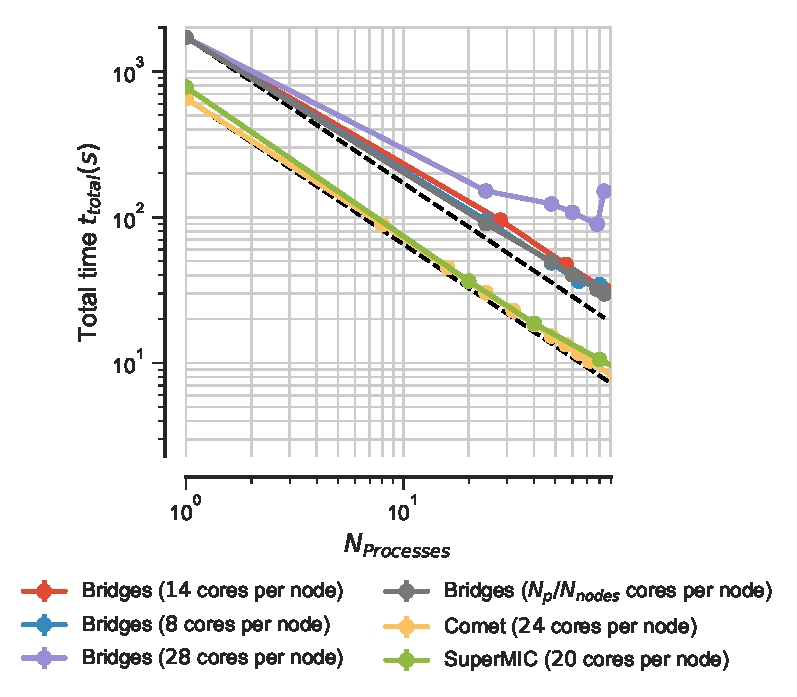
\includegraphics[width=\linewidth]{figures/Comparison_t-tot-clusters.pdf}
  \caption{Scaling total}
  \label{fig:MPIscaling-clusters}
\end{subfigure}
\hfill
\begin{subfigure}{.4\textwidth}
  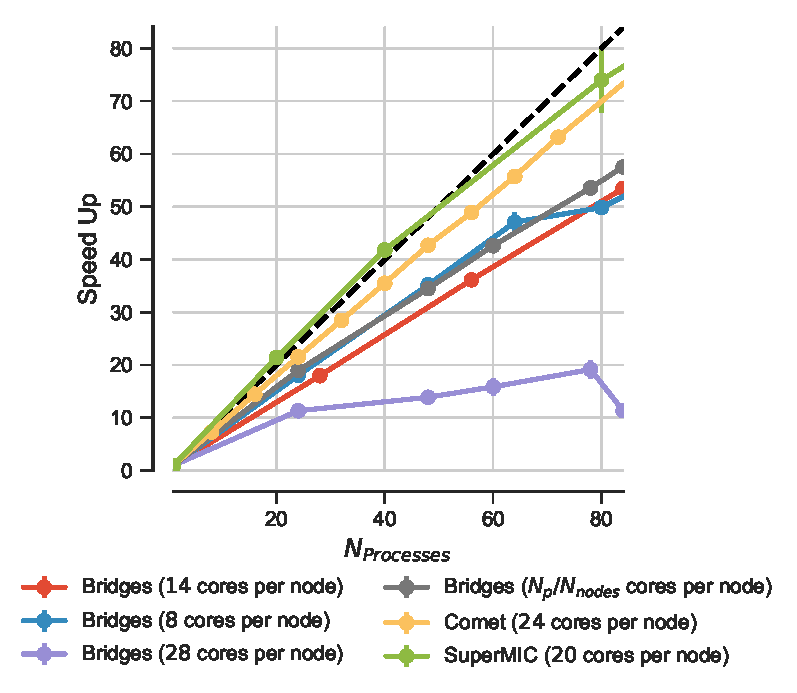
\includegraphics[width=\linewidth]{figures/Comparison_speed-up-clusters.pdf}
  \caption{Speed-up}
  \label{fig:MPIspeedup-clusters}
\end{subfigure}
\bigskip

\begin{subfigure} {.8\textwidth}
  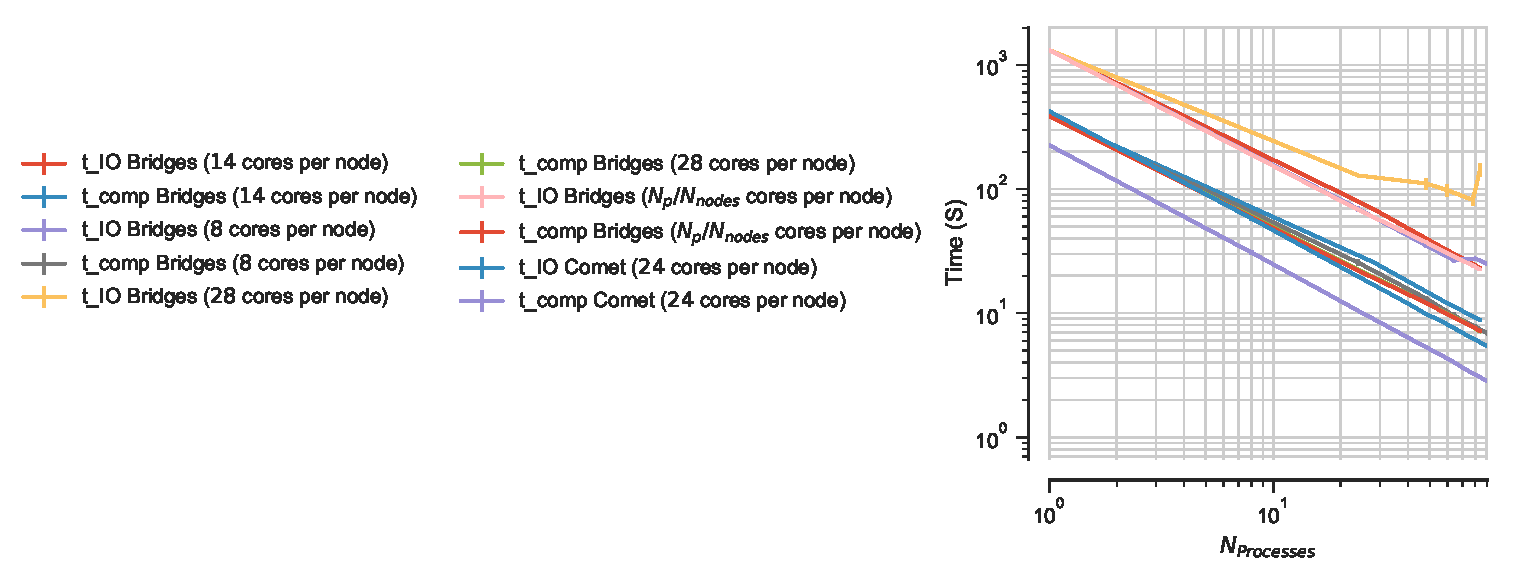
\includegraphics[width=\linewidth]{figures/Clusters_IO_compute_scaling.pdf}
  \caption{Scaling of the \tcomp and \tIO of the RMSD task with MPI-based parallel HDF5 (Independent I/O)}
  \label{fig:compute-IO-scaling-clusters}
\end{subfigure}
%
\caption{Comparison of the performance of the RMSD task with MPI ($\tcomp/\tIO \approx 0.3$)
across different clusters (SDSC Comet, PSC Bridge, SuperMIC). Data are read from a shared HDF5 file format instead of XTC format (Independent I/O)
and results are communicated back to rank 0 (communications included). Five repeats are performed to 
collect statistics. The error bars show standard deviation with respect to mean.}
\label{fig:MPIwithIO-clusters}
\end{figure} 

\begin{figure}[ht!]
\centering
\begin{subfigure}{.45\textwidth}
  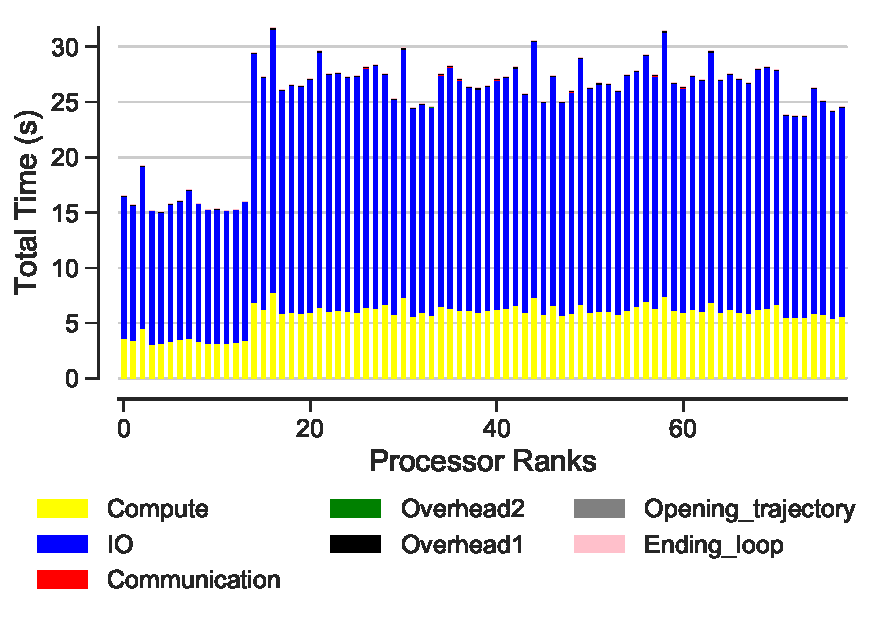
\includegraphics[width=\linewidth]{figures/Bridge-MPI-IO-BarPlot-rank-comparison_78_5.pdf}
  \caption{Bridge}
  \label{fig:hdf5-bridge}
\end{subfigure}
\bigskip
\begin{subfigure} {.45\textwidth}
  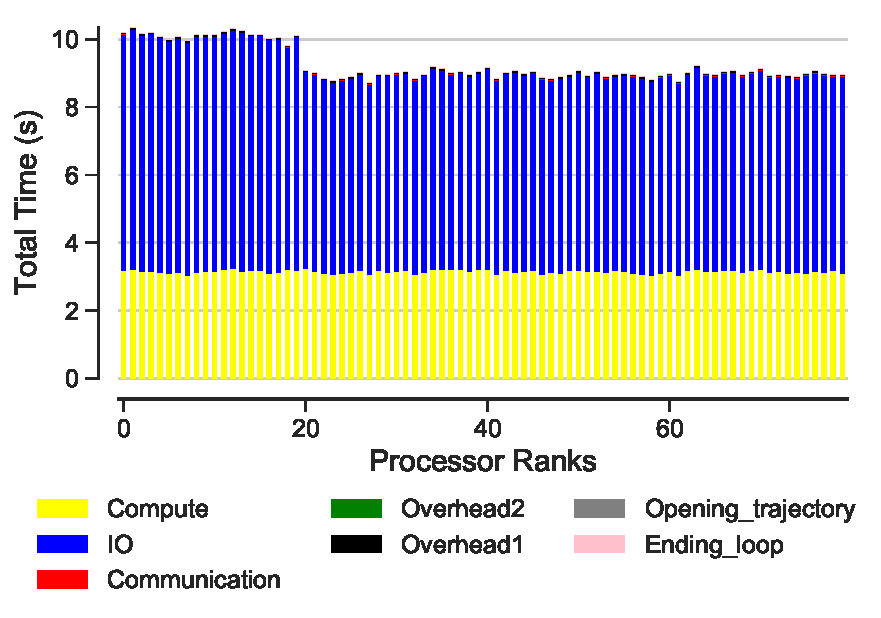
\includegraphics[width=\linewidth]{figures/SuperMIC-MPI-IO-BarPlot-rank-comparison_80_5.pdf}
  \caption{SuperMIC}
  \label{fig:hdf5-SuperMIC}
\end{subfigure}
%
\caption{Examples of timing per MPI rank for RMSD task with MPI-based parallel HDF5 ($\tcomp/\tIO \approx 0.3$) on (a) PSC Bridge and (b) SuperMIC (Buttomn).
Five repeats are performed to collect statistics and this is typical data from one run of the 5 repeats. Compute \tcomp, IO \tIO, communication \tcomm, ending the for loop $t_{end\_loop}$,
opening the trajectory $t_{opening\_trajectory}$, and overheads $t_{Overhead1}$,  $t_{Overhead2}$ per MPI rank (as described in methods).
This is typical data from one run of the 5 repeats. I/O distribution is non-uniform on Bridge while it is more uniform on SuperMIC and this explains why SuperMIC has better scaling as compared to PSC Bridge.}
\label{fig:MPIwithIO-clusters-rank}
\end{figure} 

\subsection{Comparison of Compute \& I/O Scaling Across Different Clusters}
Comparison of compute \& I/O scaling across different clusters for different test cases and algorithms is shown in Table \ref{tab:comp-IO-scaling}. 
The corresponding plots for compute and I/O scaling are shown in related sections. 
These plots together with Table \ref{tab:comp-IO-scaling} allow both quantitative and qualitative comparison of the compute and I/O time scaling.
As can be seen in Table \ref{tab:comp-IO-scaling} for MPI-based parallel HDF5, both compute and I/O time on Bridge is larger than its corresponding value on Comet and SuperMIC.
For example, with one core the corresponding compute and I/O time are about (387, 1318) versus (225, 423) and (273, 503) on Comet and SuperMIC respectively.
This performance difference becomes more obvious as the number of cores increases.
When the trajectories are splitted and global array is used for communication both Comet and SuperMIC show similar performance at small number of cores and the their performance difference increases as the number of cores increases. 
The reason why we see these performance differences is explained in previous sections. 

\begin{sidewaystable}[ht!]
\centering
\begin{adjustbox}{max width=\textwidth}
\begin{tabular}{c c c c c c c c c c c c c c}
  \toprule
 \multicolumn{10}{r}{\bfseries $N_{Processes}$} \\
\cmidrule(r){7-14}
           \bfseries\thead{Cluster} & \bfseries\thead{Calculation} & \bfseries\thead{Load Ratio} & \bfseries\thead{Gather} & \bfseries\thead{File Access} & \bfseries\thead{Time} & \bfseries\thead{1} & \begin{tabular}{c} \bfseries\thead{Comet:} 24 \\ \bfseries\thead{Bridges:} 24 \\ \bfseries\thead{SuperMIC:} 20 \end{tabular}  & \begin{tabular}{c} \bfseries\thead{Others:} 48 \\ \bfseries\thead{Bridges:} 48 \\ \bfseries\thead{SuperMIC:} 40 \end{tabular} & \begin{tabular}{c} \bfseries\thead{Comet:} 72 \\ \bfseries\thead{Bridges:} 60 \\ \bfseries\thead{SuperMIC:} 80 \end{tabular} & \begin{tabular}{c} \bfseries\thead{Comet:} 96 \\ \bfseries\thead{Bridges:} 78 \end{tabular} & \begin{tabular}{c} \bfseries\thead{Comet:} 144 \\ \bfseries\thead{Bridges:} 84 \\ \bfseries\thead{SuperMIC:} 160\end{tabular} & \bfseries\thead{Comet: 192} & \begin{tabular}{c} \bfseries\thead{Comet:} 384 \\  \bfseries\thead{SuperMIC:} 320\end{tabular}\\
  \midrule
   Comet & \makecell{Dihedral \\Featurization} & 100 & MPI & Single & \begin{tabular}{c} \tIO \\ \tcomp \end{tabular} & \begin{tabular}{c} $2880 \pm 0$ \\ $272000 \pm 0$ \end{tabular} & \begin{tabular}{c} $40 \pm 1.63$ \\ $12440 \pm 200.78$ \end{tabular} & \begin{tabular}{c} $20 \pm 1.22$ \\ $6305 \pm 38.13$ \end{tabular} & \begin{tabular}{c} $15 \pm 3.91$ \\ $4225 \pm 83.41$ \end{tabular} & -- & -- & --& --\\ 
  \midrule
    Comet & RMSD 1X & 0.3 & MPI & Single & \begin{tabular}{c} \tIO \\ \tcomp  \end{tabular} & \begin{tabular}{c} $799 \pm 5.22$ \\ $225 \pm 5.4$ \end{tabular} & \begin{tabular}{c} $49 \pm 3.45$ \\ $11 \pm 0.75$ \end{tabular} & \begin{tabular}{c} $29 \pm 1.3$ \\ $6 \pm 0.35$ \end{tabular} & \begin{tabular}{c} $26 \pm 9.19$ \\ $4 \pm 0.48$ \end{tabular} & -- & -- & -- & --\\  
  \midrule
    Comet & RMSD 1X & 0.3 & GA & Single & \begin{tabular}{c} \tIO \\ \tcomp \end{tabular} & \begin{tabular}{c} $820 \pm 18.49$ \\ $219 \pm 9.8$ \end{tabular} & \begin{tabular}{c} $41 \pm 8.99$ \\ $10 \pm 0.3$ \end{tabular} & \begin{tabular}{c} $23 \pm 4.14$ \\ $5 \pm 0.48$ \end{tabular} & \begin{tabular}{c} $15 \pm 2.06$ \\ $3 \pm 0.54$ \end{tabular} & -- & -- & -- & --\\
  \midrule
    Comet & RMSD 1X & 0.3 & MPI & Splitting & \begin{tabular}{c} \tIO \\ \tcomp \end{tabular} & \begin{tabular}{c} $799 \pm 5.22$ \\ $225 \pm 5.4$ \end{tabular} & \begin{tabular}{c} $37 \pm 1.22$ \\ $11 \pm 0.31$ \end{tabular} & \begin{tabular}{c} $18 \pm 0.18$ \\ $5 \pm 0.07$ \end{tabular} & \begin{tabular}{c} $12 \pm 0.14$ \\ $3 \pm 0.04$ \end{tabular} & \begin{tabular}{c} $9 \pm 0.3$ \\ $3 \pm 0.11$ \end{tabular} & \begin{tabular}{c} $6  \pm 0.66$ \\ $2 \pm 0.23$ \end{tabular} & \begin{tabular}{c} $4 \pm 0.23$ \\ $1 \pm 0.07$ \end{tabular} & --\\
  \midrule
    SuperMIC & RMSD 1X & 0.3 & MPI & Splitting & \begin{tabular}{c} \tIO \\ \tcomp \end{tabular} & \begin{tabular}{c} $1013.75 \pm 2.8$ \\ $304.26 \pm 2.55$ \end{tabular} & \begin{tabular}{c} $39.99 \pm 0.36$ \\ $12.41 \pm 0.22$ \end{tabular} & \begin{tabular}{c} $19.18 \pm 0.25$ \\ $5.99\pm 0.09$ \end{tabular} & \begin{tabular}{c} $9.61 \pm 0.28$ \\ $3.08 \pm 0.13$ \end{tabular} & -- & \begin{tabular}{c} $4.83 \pm 0.06$ \\ $1.5 \pm 0.01$ \end{tabular} & --& --\\ 
  \midrule 
    Comet & RMSD 1X & 0.3 & GA & Splitting & \begin{tabular}{c} \tIO \\ \tcomp \end{tabular} & \begin{tabular}{c} $820 \pm 18.5$ \\ $219 \pm 9.5$ \end{tabular} & \begin{tabular}{c} $36 \pm 0.78$ \\ $9 \pm 0.22$ \end{tabular} & \begin{tabular}{c} $17 \pm 0.3$ \\ $4 \pm 0.07$ \end{tabular} & \begin{tabular}{c} $11 \pm 0.23$ \\ $3 \pm 0.04$ \end{tabular} & \begin{tabular}{c} $10 \pm 1.7$ \\ $2 \pm 0.4$ \end{tabular} & \begin{tabular}{c} $5 \pm 0.14$ \\ $1 \pm 0.05$ \end{tabular} & \begin{tabular}{c} $4 \pm 0.07$ \\ $1 \pm 0.02$ \end{tabular} & --\\
  \midrule
    SuperMIC & RMSD 1X & 0.3 & GA & Splitting & \begin{tabular}{c} \tIO \\ \tcomp \end{tabular} & \begin{tabular}{c} $1027.62 \pm 10.32$ \\ $305.78 \pm 3.47$ \end{tabular} & \begin{tabular}{c} $39.62 \pm 0.2$ \\ $12.16 \pm 0.1$ \end{tabular} & \begin{tabular}{c} $19.66 \pm 0.1$ \\ $6.01\pm 0.007$ \end{tabular} & \begin{tabular}{c} $9.57 \pm 0.1$ \\ $2.97 \pm 0.1$ \end{tabular} & -- & \begin{tabular}{c} $4.86 \pm 0.05$ \\ $1.51 \pm 0.03$ \end{tabular} & --& --\\     
  \midrule
    Comet & RMSD 1X & 0.3 & MPI & PHDF5 & \begin{tabular}{c} \tIO \\ \tcomp \end{tabular} & \begin{tabular}{c} $423 \pm 5.88$ \\ $225 \pm 6.55$ \end{tabular} & \begin{tabular}{c} $19 \pm 0.3$ \\ $10 \pm 0.12$ \end{tabular} & \begin{tabular}{c} $9 \pm 0.13$ \\ $5 \pm 0.1$ \end{tabular} & \begin{tabular}{c} $6 \pm 0.06$ \\ $3 \pm 0.04$ \end{tabular} & \begin{tabular}{c} $5 \pm 0.12$ \\ $2 \pm 0.05$ \end{tabular} & \begin{tabular}{c} $3 \pm 0.2$ \\ $1 \pm 0.04$ \end{tabular} & \begin{tabular}{c} $3 \pm 0.25$\\ $1 \pm 0.03$ \end{tabular} & \begin{tabular}{c} $1.57 \pm 0.29$\\ $0.76 \pm 0.09$ \end{tabular}\\
  \midrule 
    Bridges & RMSD 1X & 0.3 & MPI & PHDF5 & \begin{tabular}{c} \tIO \\ \tcomp \end{tabular} & \begin{tabular}{c} $1318.87 \pm 10.42$ \\ $387.8 \pm 5.51$ \end{tabular} & \begin{tabular}{c} $67.93 \pm 0.52$ \\ $21.97 \pm 0.38$ \end{tabular} & \begin{tabular}{c} $37.37 \pm 0.2$ \\ $12.12 \pm 0.34$ \end{tabular} & \begin{tabular}{c} $30.35 \pm 0.15$ \\ $9.79 \pm 0.24$ \end{tabular} & \begin{tabular}{c} $24.16 \pm 0.89$ \\ $7.72 \pm 0.03$ \end{tabular} & \begin{tabular}{c} $22.5 \pm 0.17$ \\ $7.18 \pm 0.08$ \end{tabular} & -- & --\\ 
  \midrule
    SuperMIC & RMSD 1X & 0.3 & MPI & PHDF5 & \begin{tabular}{c} \tIO \\ \tcomp \end{tabular} & \begin{tabular}{c} $503.69 \pm 2.57$ \\ $273.54 \pm 4.7$ \end{tabular} & \begin{tabular}{c} $12.96 \pm 0.06$ \\ $23.44 \pm 0.29$ \end{tabular} & \begin{tabular}{c} $6.46 \pm 0.02$ \\ $12.22 \pm 0.43$ \end{tabular} & \begin{tabular}{c} $3.2 \pm 0.01$ \\ $7.3 \pm 0.85$ \end{tabular} & -- & \begin{tabular}{c} $1.64 \pm 0.01$ \\ $4.59 \pm 0.96$ \end{tabular} & --& \begin{tabular}{c} $0.82 \pm 0.004$ \\ $1.55 \pm 0.009$ \end{tabular} \\
  \bottomrule
\end{tabular}
\end{adjustbox}
\caption[Notation of our performance modeling]
{Comparison of the compute and I/O scaling for different test cases and number of processes. Five repeats are performed to collect statistics. The mean value and the
standard deviation with respect to mean are reported for each case.\gpnote{The font is extremely small in this table. Also can you add lines between different experiment configurations? Haven't the number of cores per node played a role to the overall performance?}\mknote{I corrected it. The number of cores per node has had effects and we need to have a discussion on that in text. Do you have any suggestion except from what I have disussed.}}
\label{tab:comp-IO-scaling}
\end{sidewaystable}



\section{Guidelines on the Parallel Analysis of Three Dimensional Time Series}
\label{guideline}
Here we provide practical guidelines for parallel analysis of the three dimensional time series (MD trajectories) on HPC resources.

\begin{description}
  \item[\textbf{Rule 1}] Calculate the value of \tcomp/\tIO to see whether the task is compute bound ($\frac{\tcomp}{\tIO} \gg 1$) or IO bound ($\frac{\tcomp}{\tIO} \ll 1$). As discussed in Section \ref{bound} for I/O bound problems both communication and I/O will be a problem and the performance of the task will be affected by the straggler tasks which delay job completion time.  
  
  \item[\textbf{Rule 2}] For $\frac{\tcomp}{\tIO} \geqslant 100$ the task is compute bound and the task will scale very well as we showed in Section \ref{DF}. However, if the size of the data to be communicated to rank 0 using the blocking collective communication ($MPI.Gather()$) is small, one might consider using global arrays to achieve near ideal scaling behavior (Section \ref{Global-Array}). In fact the overhead of \package{mpi4py} is large with respect to C for small array size \cite{Dalcin:2011aa}. Application of Global array is useful in the sense that it replaces message-passing interface with a distributed shared array where its blocks will be updated by the associated rank in the communication domain (Algorithm \ref{alg:GA}). 
  \item[\textbf{Rule 3}] For $\frac{\tcomp}{\tIO} \leqslant 100$ the task is I/O bound and then one need to take the following steps:
   
\begin{description}
  \item[\textbf{Rule 3.1}] If there is access to HDF5 format the recommended way will be to use MPI-based Parallel HDF5 (Section \ref{HDF5}). Since converting the XTC file to HDF5 is expensive if the trajectory file formats are not in HDF5 form then one might prefer to split the trajectories. MD trajectories are often re-analyzed and therefore we suggest to incorporate trajectory conversion into the beginning of standard workflows for MD simulations. 
 Alternatively, it will be a good idea to keep the trajectories in smaller chunks, e.g. when running simulations on HPC resources using Gromacs [??], users can run their simulations with ``-noappend" option which will automatically store the output trajectories in small chunks.
  \item[\textbf{Rule 3.2}] If there is not access to HDF5, the trajectory file should be splitted into as many trajectory segments as the number of processes. Splitting the trajectories is fast and does not take much time (\ref{sec:splitting-timing}).
  \item[\textbf{Rule 3.3}] The appropriate parallel implementation along with \emph{Global Array} should be used on the trajectory segments (Section \ref{Splitting}) to achieve near ideal scaling.
\end{description}
\end{description}


\section{Conclusion}
\label{concl} 
There are currently many freely available libraries for the analysis and processing of molecular dynamics trajectories.
However, dramatic increases in the size of trajectories combined with the serial nature of these libraries necessitates 
use of state of the art high performance computing tools for rapid analysis of these time series. 

\package{MDAnalysis} is a package for post-processing of MD trajectories; however, it does not currently provide parallel analysis of these trajectories.
In this study, we looked at the \emph{straggler} problem that we previously faced in an attempt for parallel analysis of these trajectories in \package{MDAnalysis} \cite{Khoshlessan:2017ab}.
To this aim, we tested our benchmark on RMSD (I/O bound) algorithm in \package{MDAnalysis}.

Our initial analysis showed that the ratio between compute load to I/O load and compute load to communication load have a crucial effect on the performance. 
For sufficiently large per-frame workloads ($\tcomp/\tIO \approx 100$), close to ideal scaling was achievable (Figure \ref{fig:comparison-t_comm-dihedral}).
However, the I/O bound workload ($\tcomp/\tIO \approx 0.3$) does not scale due to the appearance of \emph{stragglers}. 

Different factors like opening the trajectory file, or other sources of overheads can be responsible for observing \emph{stragglers} for I/O bound workload.
But, for the I/O bound workload, both communication and I/O appeared to be the main scalability bottlenecks when using a shared file.
Our data suggest that \emph{stragglers might be due to the competition between MPI and the Lustre file system on the shared Infini-band interconnect}.  
Since I/O traffic must compete with MPI messages and other traffics, it can be difficult to achieve peak single-node I/O rates for an arbitrary file when the system is fully loaded with other jobs \cite{VMD2013, Kevin2018}. 

This is because when we remove I/O, communication does not appear to be the scalability bottleneck anymore (data not shown here).
In fact, communication time, \tcomm, could take
much longer for \emph{stragglers} than for ``normal'' MPI ranks when I/O has to be performed through a shared trajectory file (Figure \ref{fig:MPIranks}). 

Additionally, the number of I/O requests is a function of number of frames in the trajectory. 
For I/O bound task and compute bound task with the same number of frames per trajectory, the frequency of sending the I/O requests makes a difference.
For sufficiently large per-frame compute workload, the I/O requests interfere much less often with communication than an I/O bound task.
\obnote{citations? How can you back up this statement?}\mknote{Our results sugest. When we increse workload we see this effect right?}
This is why both communication and I/O appeared to prevent us from achieving the near ideal scaling for an I/O bound task.

It should be also noted that, for $\frac{\tcomp}{\tcomm} \gg 1$ and $\frac{\tcomp}{\tIO} \gg 1$, the effect of communication was less pronounced when the work became more compute-bound and this 
is because with compute-bound tasks there is less competition over accessing the shared trajectory file.
We showed this effect by changing the ratio between compute load and I/O load and studying its impact on the performance.

Therefore, for I/O bound tasks we needed to come up with solution to overcome \emph{stragglers}. 
We were able to achieve much better performance in our RMSD benchmark when we used global array toolkit instead of message-passing interface for communication. 
Using global array, we did not observe any delayed task due to communication (Figure \ref{fig:MPIwithIO-ga4py}) and it significantly reduced the communication cost. 
However, reducing communication cost was not enough for achieving near ideal scaling because I/O remains a bottleneck.

We showed several approaches to improve I/O scaling.
We were able to improve I/O through splitting the shared trajectory file (Figure \ref{fig:MPIwithIO-split}) and MPI-based parallel I/O through HDF5 file (Figure \ref{fig:MPIwithIO-hdf5}). 
\obnote{future: adopt the mdtraj HDF5 format http://mdtraj.org/latest/hdf5\_format.html (and cite mdtraj paper)}\mknote{Which part do you mean?}
In both cases, we were able to achieve near ideal scaling.
With splitting the trajectories, effect of communication is still apparent on the performance which is because $\frac{\tcomp}{\tcomm} \ll 1$; however together with 
global array toolkit we could achieve near ideal scaling (Figure \ref{fig:MPIwithIO-split}).
\obnote{I actually do not understand why we need GA for splitting but not for parallel MPI.}
\mknote{I mentioned before in my presentation in Spidal meeting that I myself do not have an answer for this.}

All the above strategies, provide guidelines for parallel analyses on data generated from MD simulations in \package{MDAnalysis} library.
The analysis indicates that splitting the trajectories in combination with global array or parallel I/O will make it feasible to run an I/O bound task on scalable computers up to 8 nodes and achieve near ideal scaling behavior.
In addition, we have examined all these benchmarks on several HPC resources in order to show the robustness of our approach.

\footnotesize{{\it Acknowledgements} Funding: This work was supported
  by the National Science Foundation [grant numbers
  1443054,1440677]. Computational resources were provided by NSF XRAC
  awards TG-MCB090174 and TG-MCB130177.

\section*{References}

\bibliography{journals,becksteinlab,sp,md,stragglers-papers,Stragglers}

\clearpage

\appendix
\section{Detailed timing for splitting the trajectories}
\label{sec:splitting-timing}
\paragraph{Detailed timing for splitting the trajectories}

Table \ref{tab:timing-splitting} shows the necessary time for splitting the trajectory file using MPI on SDSC Comet.
 
\begin{table}
\centering
\begin{tabular}{c c c}
  \toprule
            \thead{Number of trajectory segments} & \thead{$N_{p}$ used for writing the segments} & \thead{time (s)}\\
  \midrule
    $24$ & $24$ & 89.92\\
    $48$ &  $48$ & 46.79 \\
    $72$ &  $72$ & 33.7 \\
    $96$ & $96$ & 25.12\\
    $144$ & $144$ & 43.7 \\
    $196$ &  $196$ & 13.49 \\  
  \bottomrule
\end{tabular}
\caption[Time necessary for writing the trajectory segments]
{The wall-clock time spent for writing $N_{p}$ trajectory segments using $N_{p}$ processes using MPI on SDSC Comet}
\label{tab:timing-splitting}
\end{table}


\paragraph{Version of the libraries used for the present study}

Information regarding the version of each library used for the present study is given in Table \ref{tab:version}. 

\begin{table}
\centering
\begin{tabular}{c c}
  \toprule
            \thead{Package} & \thead{Version}\\
  \midrule
    PHDF5 & 1.10.1\\
    h5py &  2.7.1 \\
    GA4py & 1.0 \\
    Global Array & 5.6.1\\
    MDAnalysis & 0.17.0 \\
  \bottomrule
\end{tabular}
\caption[Version of the packages used in the present study]
{Version of the packages used in the present study}
\label{tab:version}
\end{table}

\section{Python codes used for the benchmark study}
\label{sec:codes}
\subsection{Python code used for \emph{RMSD} task with MPI for Python}
\label{sec:codeRMSD}

\begin{python}
import sys
import numpy as np
import MDAnalysis as mda
from MDAnalysis.analysis import rms
import time
from shutil import copyfile
import glob, os
import mpi4py
from mpi4py import MPI
#---------------------------------------
MPI.Init

comm = MPI.COMM_WORLD
size = comm.Get_size()
rank = comm.Get_rank()
#------------------------------------------
j = sys.argv[1]

def block_rmsd(index, topology, trajectory, xref0, start=None, stop=None, step=None):
    clone = mda.Universe(topology, trajectory)
    g = clone.atoms[index]

    bsize = int(stop-start)
    results = np.zeros([bsize,2], dtype=float)
  
    for iframe, ts in enumerate(clone.trajectory[start:stop:step]):
        results[iframe, :] = ts.time, rms.rmsd(g.positions, xref0, center=True, superposition=True)

    return results
#-----------------------------------------------------------------------
# Check the files in the directory
PSF = os.path.abspath(os.path.normpath(os.path.join(os.getcwd(),'files/adk4AKE.psf')))
longXTC = os.path.abspath(os.path.normpath(os.path.join(os.getcwd(),'newtraj.xtc')))
longXTC1 = os.path.abspath(os.path.normpath(os.path.join(os.getcwd(),'files/newtraj{}.xtc'.format(j))))

if rank == 0:
   copyfile(longXTC, longXTC1)
   u = mda.Universe(PSF, longXTC1)
   print(len(u.trajectory))

MPI.COMM_WORLD.Barrier()
#----------------------------------------------------------------------
u = mda.Universe(PSF, longXTC1)
mobile = u.select_atoms("(resid 1:29 or resid 60:121 or resid 160:214) and name CA")[1:147]
index = mobile.indices
topology, trajectory = mobile.universe.filename, mobile.universe.trajectory.filename
ref0 = mobile
xref0 = ref0.positions-ref0.center_of_mass()

# Create each segment for each process
frames_seg = np.zeros([size,2], dtype=int)
bsize = int(np.ceil(mobile.universe.trajectory.n_frames / float(size)))
for iblock in range(size):
    frames_seg[iblock, :] = iblock*bsize, (iblock+1)*bsize

d = dict([key, frames_seg[key]] for key in range(size))

start, stop = d[rank][0], d[rank][1]

# Block-RMSD in Parallel
out = block_rmsd(index, topology, trajectory, xref0, start=start, stop=stop, step=1)

if rank == 0:
   data1 = np.zeros([size*bsize,2], dtype=float)
else:
   data1 = None

comm.Gather(out[0], data1, root=0)

if rank == 0:
   data = np.zeros([size,5], dtype=float)
else:
   data = None

comm.Gather(np.array(out[1:], dtype=float), data, root=0)

MPI.Finalize                                                                                                                                                 
\end{python}

\subsection{Python code used for \emph{RMSD} task using global array with MPI for Python.}
\label{sec:codeRMSD-ga}

\begin{python}
import sys
import numpy as np
import MDAnalysis as mda
from MDAnalysis.analysis import rms
import time
from shutil import copyfile
import glob, os
import mpi4py
from mpi4py import MPI
from ga4py import ga
from ga4py import gain
#---------------------------------------
ga.initialize()
comm = gain.comm()

size = ga.nnodes()
rank = ga.nodeid()
#------------------------------------------
j = sys.argv[1]

def block_rmsd(index, topology, trajectory, xref0, start=None, stop=None, step=None):
    clone = mda.Universe(topology, trajectory)
    g = clone.atoms[index]

    print("block_rmsd", start, stop, step)
    bsize = int(stop-start)
    results = np.zeros([bsize,2], dtype=float)

    for iframe, ts in enumerate(clone.trajectory[start:stop:step]):
        results[iframe, :] = ts.time, rms.rmsd(g.positions, xref0, center=True, superposition=True)

    return results
#---------------------------------------------------------------------------
PSF = os.path.abspath(os.path.normpath(os.path.join(os.getcwd(),'files/adk4AKE.psf')))
longXTC = os.path.abspath(os.path.normpath(os.path.join(os.getcwd(),'newtraj.xtc')))
longXTC1 = os.path.abspath(os.path.normpath(os.path.join(os.getcwd(),'files/newtraj{}.xtc'.format(j))))

if rank == 0:
   copyfile(longXTC, longXTC1)
   u = mda.Universe(PSF, longXTC1)
   print(len(u.trajectory))

ga.sync()
#----------------------------------------------------------------------
u = mda.Universe(PSF, longXTC1)
mobile = u.select_atoms("(resid 1:29 or resid 60:121 or resid 160:214) and name CA")
index = mobile.indices
topology, trajectory = mobile.universe.filename, mobile.universe.trajectory.filename
ref0 = mobile
xref0 = ref0.positions-ref0.center_of_mass()
bsize = int(np.ceil(mobile.universe.trajectory.n_frames / float(size)))
g_a = ga.create(ga.C_DBL, [bsize*size,2], "RMSD")
buf = np.zeros([bsize*size,2], dtype=float)

# Create each segment for each process
frames_seg = np.zeros([size,2], dtype=int)
bsize = int(np.ceil(mobile.universe.trajectory.n_frames / float(size)))
for iblock in range(size):
    frames_seg[iblock, :] = iblock*bsize, (iblock+1)*bsize

d = dict([key, frames_seg[key]] for key in range(size))

start, stop = d[rank][0], d[rank][1]

# Block-RMSD in Parallel
out = block_rmsd(index, topology, trajectory, xref0, start=start, stop=stop, step=1)

ga.put(g_a, out[0][:,:], (start,0), (stop,2))

if rank == 0:
   buf = ga.get(g_a, lo=None, hi=None)

if rank == 0:
   data = np.zeros([size,5], dtype=float)
else:
   data = None

comm.Gather(np.array(out[1:], dtype=float), data, root=0)
                 
ga.destroy(g_a)
ga.terminate()
\end{python}

\subsection{Python code used for \emph{Dihedral Featurization} task with MPI for Python}
\label{sec:codeDihed}

\begin{python}
import MDAnalysis as mda
import numpy as np
import glob
from itertools import chain
import time
from shutil import copyfile
import glob, os
import mpi4py
from mpi4py import MPI
import sys
#---------------------------------------
MPI.Init

comm = MPI.COMM_WORLD
size = comm.Get_size()
rank = comm.Get_rank()
#------------------------------------------
j = sys.argv[1]

def angle2sincos(x):
    """Convert angle x to (cos x, sin x).
    
    Parameters
    ----------
    x : float or array_like
    
    Returns
    -------
    feature_vector : array
        1D feature vector ``[cos(x[0]), sin(x[0]), cos(x[1]), sin(x[1]), ...]``.
    """
    x = np.deg2rad(x)
    return np.ravel(np.transpose([np.cos(x), np.sin(x)]))

def residues_to_dihedrals(residues):
    """Return list of [phi1, psi1, phi2, psi2, ...] dihedral objects"""
    return list(chain.from_iterable(
            (res.phi_selection().dihedral, res.psi_selection().dihedral) for res in residues))

def featurize_dihedrals(dihedrals):
    angles = [dihedral.value() for dihedral in dihedrals]
    return angle2sincos(angles)
    
def block_dihedrals(index, topology, trajectory, start=None, stop=None, step=None):
    start00 = time.time()
    clone = mda.Universe(topology, trajectory)
    g = clone.atoms[index]
    residues = g.residues[1:-1]
    dihedrals = residues_to_dihedrals(residues)

    print("block_rmsd", start, stop, step)
    print(len(clone.trajectory))
    bsize = stop-start
    results = []

    for iframe, ts in enumerate(clone.trajectory[start:stop:step]):
        results.append(featurize_dihedrals(dihedrals))

    return np.array(results)
#----------------------------------------------------------------------
PSF = os.path.abspath(os.path.normpath(os.path.join(os.getcwd(),'files/adk4AKE.psf')))
longXTC = os.path.abspath(os.path.normpath(os.path.join(os.getcwd(),'newtraj.xtc')))
longXTC1 = os.path.abspath(os.path.normpath(os.path.join(os.getcwd(),'files/newtraj{}.xtc'.format(j))))

if rank == 0:
    copyfile(longXTC, longXTC1)
    u = mda.Universe(PSF, longXTC1)
    print(len(u.trajectory))

MPI.COMM_WORLD.Barrier()
#----------------------------------------------------------------------
u = mda.Universe(PSF, longXTC1)
mobile = u.select_atoms("protein")
index = mobile.indices

topology, trajectory = mobile.universe.filename, mobile.universe.trajectory.filename
bsize = int(np.ceil(mobile.universe.trajectory.n_frames / float(size)))

# Create each segment for each process
frames_seg = np.zeros([size,2], dtype=int)
bsize = int(np.ceil(mobile.universe.trajectory.n_frames / float(size)))
for iblock in range(size):
    frames_seg[iblock, :] = iblock*bsize, (iblock+1)*bsize

d = dict([key, frames_seg[key]] for key in range(size))

start, stop = d[rank][0], d[rank][1]

out = block_dihedrals(index, topology, trajectory, start=start, stop=stop, step=1)

if rank == 0:
   data1 = np.zeros([size*bsize,848], dtype=float)
else:
   data1 = None

comm.Gather(out[0], data1, root=0)

if rank == 0:
    data = np.zeros([size,5], dtype=float)
else:
    data = None

comm.Gather(np.array(out[1:], dtype=float), data, root=0)

MPI.Finalize   
\end{python}

\end{document}